\chapter{Theory}
\label{chap:theory}
%\begin{quote}
% \textit{This chapter discusses the theory of energy transfer.}
%\end{quote}

This chapter is devoted to the theory and methods used in this thesis. Section \ref{sec:theory} presents the relevant equations for describing phononic, electronic and photonic energy transfer in microscopic scale, aiming at giving a unified, parallel treatment of the three carriers. Because earlier parallel treatments (see, e.g., Ref. \cite{chen}) of the three carriers have mostly stressed the analogies in the energy transfer phenomena, we stress here the similarity of the Langevin equations of motion. The Langevin terms capture both thermal fluctuations and dissipation, necessary in modeling the creation and annihilation of energy carriers. 

Section \ref{sec:methods} discusses the methods used for solving the equations of motion. 

% We first review the classical molecular dynamics method, which was used to investigate lattice heat transfer in different geometries. Molecular dynamics allows for including non-linearities in the equations of motion, thereby accounting for detailed phonon-phonon interactions between different modes. Second approach to solving the equations of motion is the Green's function method, which requires, however, that the equations are fully linear \footnote{Keldysh Green's function methods \cite{haugjauho,wang08} can be used for perturbatively including non-linearities, but they are computationally heavy and therefore applicable only for relatively small systems.}. In this case, dissipative processes are captured by the effective relaxation rates introduced by the Langevin baths. The solution of Langevin equations of motion in terms of Green's functions is very similar for all three carriers, so the treatment is kept general when possible.
 
% Methods

% The role of Langevin baths

% 

\section{Theory of energy transfer}
\label{sec:theory}

This section discusses the theory of lattice vibrations, electromagnetic field, and electron transport. The equations of motion of the three carriers are presented in Sec. \ref{sec:th_eom}, starting from emphasizing the similarities of linearized Langevin equations of motion constituting a minimal (and often sufficient) model for energy transfer. Discussion of the general equations of motion is postponed to Sec. \ref{sec:th_eom2}. The presented equations of motion generally consist of deterministic terms derivable from microscopic Hamiltonians and Langevin force terms. The Langevin terms describe both the creation and annihilation of carriers necessary in transport modeling. The properties of the Langevin baths for the three carriers are discussed in detail in Sec. \ref{sec:th_langevin}.  

% For generality, we include both deterministic terms derivable from microscopic Hamiltonians and external force terms arising from interaction with stochastic Langevin baths. The stochastic fluctuations induced by the baths act as source terms in the equations, driving energy transfer. Fluctuation-dissipation theorem requires the fluctuations to be accompanied by friction terms, damping carriers and thereby introducing dissipation. 

\subsection{Equations of motion: parallel treatment}
\label{sec:th_eom}

\begin{figure}
 \begin{center}
 \end{center}
 \caption{Schematic illustration of microscopic energy transfer mechanisms: (a) vibrational, (b) electromagnetic, and (c) electronic energy transfer.}
 \label{fig:mechanisms}
\end{figure}

This subsection summarizes the minimal equations of motion governing vibrational, electromagnetic and electronic energy transfer. These stochastic equations of motion allow for fully quantum-mechanical derivation of energy transfer rates and account for wave effects and also for dissipation at the level of one-particle relaxation rates. These microscopic, Langevin equations of motion for vibrational, electromagnetic and electronic energy transfer originate, respectively, from the works of Bolsterli, Rich and Visscher \cite{bolsterli70}, Rosa, Dalvit and Milonni \cite{rosa10,rosa11}, and Dhar and Roy \cite{dhar03}. In this thesis, we show how these, so far unconnected, equations allow for calculation of spectral energy transfer rates in terms of Green's functions. More general equations are presented below in Sec. \ref{sec:th_eom2}, where also the steps leading to the minimal equations are presented and more references are given.

Different energy transfer mechanisms and the relevant degrees of freedom are schematically illustrated in Fig. \ref{fig:mechanisms}. Vibrational heat transfer in solids arises from the displacements $\bu_i$ of atoms from their equilibrium positions. The displaced atoms exerts forces on other atoms, thereby leading to energy transfer. Similarly, electromagnetic energy transfer is intervowen with the dynamics of local dipole moments $\bp_i=q\bd_i$, where $q$ is the dipole charge and $\bd_i$ the dipole displacement. An oscillating dipole radiates electromagnetic energy, which is absorbed by other dipoles. Electron dynamics can be described in the tight-binding picture \cite{} by electrons hopping between orbitals. Mathematically, the dynamics of a fixed number of electrons is described by the Schr\"odinger equation for electron wavefunction \cite{griffiths_qm}, but to capture fluctuations and dissipation leading to  electron creation and annihilation, it is more practical to consider the dynamics of Fock operators $c_i^{\dagger}$ and $c_i$ \cite{ballentine} creating and and annihilating electrons at orbital $i$, respectively (spin indices are suppressed throughout). For notational simplicity, the same subindex $i$ is used for different degrees of freedom, but they are not necessarily related. 

In the linear approximation, the equations of motion for the three degrees of freedom are, respectively, \cite{bolsterli70,rosa10,rosa11,dhar03}
\begin{subequations}
\begin{align}
 m_i \ddot{\bu}_i(t) &=  - \sum_j \bb{K}_{ij}\bb{u}_j(t) + \xi_i(t) - m_i \gamma \dot{\bu}_i, \label{eq:th_eom1} \\
 m \ddot{\bb{d}}_i(t) &= - m\omega_0^2 \bb{d}_i(t) + q\sum_{j} \bb{E}_{ij}(t)+\xi_i(t) - m_i \gamma \dot{\bu}_i(t), \label{eq:th_eom2}\\
 i\hbar \dot{c}_i(t) &= -\sum_j t_{ij} c_j(t) +\eta_i(t) - i\hbar \gamma_e c_i(t) \label{eq:th_eom3}.
\end{align}
\end{subequations}
The approximations leading to these equations are discussed in detail below in Sec. \ref{sec:th_eom2}, where also all the quantities are defined and the relevant references for these equations are given. These equations can, however, be easily understood intuitively. As an example, Eq. \eqref{eq:th_eom1} states that the acceleration of atom $i$ is proportional to the sum of (i) the forces exerted by other atoms $j$, proportional for each atom pair $i,j$ to the force constant matrix $\bb{K}_{ij}$ defined below, (ii) stochastic Langevin force $\xi_i$ generating thermal fluctuations, and (iii) Langevin friction $m_i \gamma \dot{\bu}_i$ responsible for dissipation. The assumption of a linear interparticle force is relaxed below in Sec. \ref{sec:th_eom2} to allow for more exact treatment of non-linear forces, necessary in the calculation of, e.g., frequency-dependent mean free paths. The variance of the fluctuating force $\xi_i$ and the friction constant $\gamma$ are related by the fluctuation-dissipation theorem presented in Sec. \ref{sec:th_langevin}. 

Equation of motion \eqref{eq:th_eom2} for the dipole moment $\bb{d}_i$ is similar to Eq. \eqref{eq:th_eom1}, but here the force exerted by other dipoles $j$ is mediated by the electric fields $\bE_{ij}$. The relation of this dipole equation of motion to the more commonly used fluctuating electrodynamics \cite{} is discussed in Sec. \ref{sec:th_eom2}. In the Heisenberg equation of motion \eqref{eq:th_eom3} for electron annihilation operator, on the other hand, the dynamics of different orbitals are coupled by the tight-binding hopping constant $t_{ij}$ allowing for electron hopping between orbitals.

Steady-state solution of Eqs. \eqref{eq:th_eom1}-\eqref{eq:th_eom3}, independent of initial conditions, can be found \cite{chaikin} by Fourier transforming the equations. We define Fourier transformation for any function $f(t)$, as usual, as \cite{chaikin}
\begin{equation}
 \tilde f(\omega) = \int_{-\infty}^{\infty} dt e^{i\omega t} f(t)
\end{equation}
and the corresponding inverse transformation as
\begin{equation}
 f(t) = \int_{-\infty}^{\infty} \frac{d\omega}{2\pi} e^{-i\omega t}\tilde f(\omega).
\end{equation}
Here $\omega$ is the angular frequency. Fourier transformation and expanding the electric field term $\bE_{ij}$ in Eq. \eqref{eq:th_eom2} as described in Sec. \ref{sec:th_eom2} leads to the linear system of equations
\begin{subequations}
\begin{align}
   - & \sum_{j,\beta}  [m_i (\omega^2+i\gamma \omega) \delta_{ij}\delta^{\alpha\beta} - K_{ij}^{\alpha\beta}] \tilde{u}_j^{\beta}(\omega) = \tilde \xi_i^{\alpha}(\omega) \label{eq:th_eom_fourier_phonon} \\
  - &  \sum_{j,\beta} \left[m(\omega^2-\omega_0^2+i\gamma\omega) \delta_{ij}\delta_{\alpha\beta} +q^2 \omega^2 \mu_0 \mathbb{G}^{\alpha\beta}(\br_i,\br_j;\omega) \right]\tilde{d}_j^{\beta}(\omega) \notag \\
  & \qquad = q\tilde{E}_{0,i}^{\alpha}(\omega) + \tilde{\xi}^{\alpha}_i(\omega) \label{eq:th_eom_fourier_photon} \\ 
  &  \sum_{j} \left[\hbar (\omega+i\gamma_e) \delta_{ij} + t_{ij} \right] \tilde c_j(\omega) = \tilde \eta_i(\omega)   \label{eq:th_eom_fourier_electron}
\end{align}
\end{subequations}
In Eq. \eqref{eq:th_eom_fourier_photon}, the electromagnetic Green's dyadic $\mathbb{G}^{\alpha\beta}$ \cite{novotny} couples different dipoles and $E_{0,1}^{\alpha}$ is the background electric field. Each of these equations can be written in the matrix form
%he equations of motion \eqref{eq:th_eom_phonon_fourier}, \eqref{eq:th_eom_electron} and \eqref{eq:th_eom_dipoles} generally reduce to the matrix form
\begin{equation}
 \bb{A}(\omega) \tilde{\bb{x}}(\omega) = \sum_J \tilde \zeta^J(\omega). \label{eq:th_general}
\end{equation}
where $\bb{A}(\omega)$ is a coefficient matrix multiplying the degrees of freedom $\tilde{\bb{x}}(\omega)$ (standing for $\bu$, $\bb{c}$, or $\bb{d}$ written in vector form) and the right-hand side is the sum over stochastic Langevin forces $\zeta^J$ (standing for $\xi^J$ or $\eta^J$) from each bath $J$. To arrive at the matrix form, we have combined the site indices and coordinates into a single composite index. The bath index $J$ typically includes the baths coupled to each atomic site in the scattering region and, in case of phonons and electrons, baths representing external leads, which themselves consist of atoms coupled to Langevin baths at a prescribed temperature (and chemical potential for electrons). 

To illustrate the solution of Eq. \eqref{eq:th_general}, let us define the Green's function as the matrix inverse $\bb{G}(\omega)=\bb{A}(\omega)^{-1}$ so that  
\begin{equation}
 \tilde{\bb{x}}(\omega)  = \sum_J \bb{G}(\omega)\tilde \zeta^J(\omega). \label{eq:th_gf_solution}
\end{equation}
Equation \eqref{eq:th_gf_solution} can be straightforwardly interpreted: system's dynamics at frequency $\omega$ originates from the stochastic fluctuations from each bath (corresponding to carrier generation), with the Green's function acting as the transfer matrix. The Green's function itself is generally of the form
\begin{equation}
 \bb{G}(\omega) = \left[\bb{G}^0(\omega)^{-1} - \sum_J \Sigma^J(\omega) \right]^{-1},
\end{equation}
where $\bb{G}^0(\omega)$ is the Green's function in absence of dissipation (i.e., Langevin baths) and bath self-energy matrices $\Sigma^J(\omega)$ correspond to dissipation (corresponding to carrier annihilation) and energy level modifications arising from the interaction with each bath $J$. For example, for the friction term $m\gamma \dot{\bu}_k$, the self-energy matrix is $[\Sigma^J(\omega)]_{ij}=-im\gamma \omega \delta_{ij} \delta_{ik}$. With the fluctuation-dissipation theorem for the force variances $\langle \zeta^J(\omega) \zeta^J(\omega')^T \rangle$ presented in Sec. \ref{sec:th_langevin} and the solution \eqref{eq:th_gf_solution} available, one can calculate the thermal averages of any observable of interest. For example, the heat current to bath $I$, which could be the locally dissipated power or the heat current flowing to the leads, is generally given by the expression
\begin{equation}
 \langle Q^I \rangle = \int_0^{\infty} \frac{d\omega}{2\pi} \hbar \omega \ca{T}_{IJ}(\omega) \left[ f_{\textrm{BE}}(\omega,T_J)- f_{\textrm{BE}}(\omega,T_I)\right],
\end{equation}
where the transmission function between baths $I$ and $J$ is defined as
\begin{equation}
 \ca{T}_{IJ}(\omega) = \textrm{Tr}\left[\Gamma^I(\omega) \bb{G}(\omega) \Gamma^J(\omega) \bb{G}(\omega)^{\dagger} \right]. \label{eq:th_caroli}
\end{equation}
Equation \eqref{eq:th_caroli} is the well-known Caroli form for the transmission function \cite{caroli71}, originally derived for ballistic two-terminal electron transport and later for phonons \cite{mingo06,yamamoto06}. In \citepub{dipole}, Eq. \eqref{eq:th_caroli} was shown to be valid also for electromagnetic energy transfer between a collection of dipoles.

%\begin{subequations}
%\begin{align}
% m_i \ddot{\bu}_i &=  \bb{F}_i + \xi_i - m_i \gamma \dot{\bu}_i \\
% m \ddot{\bb{d}}_i &= - m\omega_0^2 \bb{d}_i + q\bb{E}_i+\xi_i - m_i \gamma \dot{\bu}_i \\
% i\hbar \dot{c}_i(t) &= -i\left[c_i,\ca{H}_{e}\right] +\eta_i - i\hbar \gamma_e c_i(t) 
%\end{align}
%\end{subequations}


%The similarities of the equations of motion become more apparent in the linear approximation, which is discussed in more detail below. In this case, the force acting on atom $i$ becomes $F_i^{\alpha}=-\sum_{j}\sum_{\beta} K_{ij}^{\alpha\beta}u_j^{\beta}$ and the electron Hamiltonian 
\subsection{Equations of motion: separate treatment}
\label{sec:th_eom2}

This subsection is devoted to a more in-depth discussion of the equations of motion. While the linearized Langevin equations of motion \eqref{eq:th_eom1}-\eqref{eq:th_eom3} act as a good starting point for energy transfer calculations, more sophisticated modeling is needed if the microscopic dynamics is to be treated more accurately. For the calculation of phonon mean free paths, for example, the detailed anharmonic interactions must be included in the model. % The non-linearity of the equations of motion then forbids the direct solution of the equations of motion, so one has to resort to molecular dynamics simulations \cite{allentildesley} or perturbative first-principles calculations \cite{ziman}. 

We start the discussion with vibrational heat transfer, where the general equations of motion, linearization of the equations and the definition of a phonon are introduced. We then continue to the electronic transport, where the tight-binding model is introduced. Because electronic transport plays a small role in this thesis, we only consider non-interacting electrons in order to keep the discussion brief. 

Finally, we present the microscopic theory of electromagnetic energy transfer, starting from the Maxwell's equations of motion for the electric and magnetic fields. We show how the electric polarization acts as source term giving rise to thermal radiation. We also introduce the microscopic dipole model of Rosa, Dalvit and Milonni \cite{rosa10,rosa11} and compare it with the more traditional continuum electrodynamics acting as a basis for fluctuational electrodynamics \cite{}. 

\subsubsection{Phonons}

\label{sec:th_phonons}

\begin{figure}
\begin{center}
 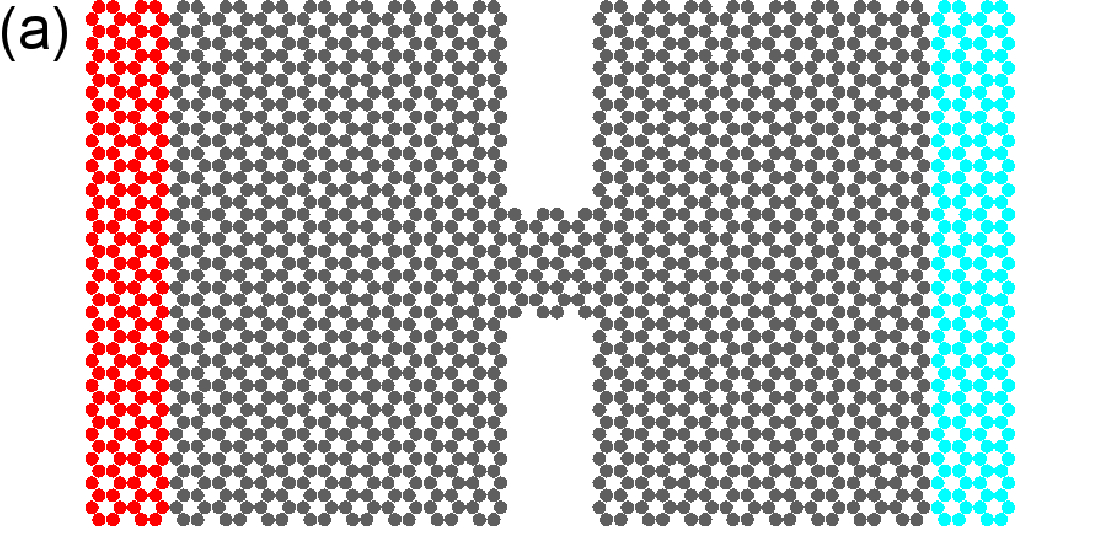
\includegraphics[width=8.6cm]{pics/gf_fig8a_2.pdf}
 \caption{Schematic illustration of a point contact in graphene. The atoms colored in red and cyan are assumed to be coupled to a heat source and sink, respectively, driving heat current through the point contact in the center region (gray atoms). In an actual calculation, the thermalized regions extend much further away from the center region.}
\label{fig:graphene_geom}
\end{center}
\end{figure} 

As a concrete example of a phonon heat transfer problem, consider the constriction in graphene, depicted in Fig. \ref{fig:graphene_geom}. Graphene is a single sheet of carbon atoms arranged in a honeycomb lattice. The rigid $sp^2$ bonding of atoms and low defect density gives rise to high thermal conductivity \cite{ghosh08,balandin11}, making graphene an attractive material for extracting heat from electronic devices \cite{yan12}. In the shown geometry, the atoms colored in red and cyan are assumed to act as heat sources and sinks at high and low temperature, respectively. The thermalized regions are assumed extend much further away from the constriction than shown in the figure. 

The theoretical description of lattice heat transfer is based on the dynamical equations of motion for the atoms constituting the lattice. The equations of motion are generally dictated by the lattice Hamiltonian \cite{ziman}
\begin{equation}
 \ca{H}_{\textrm{ph}} = \sum_{i=1}^N \frac{\bb{p}_i^2}{2m_i} + \ca{V}(\bb{r}_1,\dots,\bb{r}_N). \label{eq:th_hamiltonian}
\end{equation}
Here $\br_i$, $\bp_i$, and $m_i$ are the position, momentum and mass of atom $i$, respectively. The total number of atoms (which can also be infinite) is denoted by $N$. The first term of Eq. \eqref{eq:th_hamiltonian} is the total kinetic energy of the atoms and the second term $\ca{V}$ is the interatomic potential energy responsible for the interatomic interactions. The choice of the potential energy function $\ca{V}$ is crucial for an accurate description of the lattice dynamics and, consequently, of energy transfer. Models for $\ca{V}$ used in this work are explained in conjunction with the corresponding results.

Applying Hamilton's equations of motion $m\ddot{\br}_i=-\partial \ca{H}_{\textrm{ph}}/\partial \br_i$ \cite{fetter} accompanied by stochastic Langevin terms (discussed below) gives the equations of motion
\begin{equation}
 m_i \ddot{\br}_i(t) = \bb{F}_i(t) + \xi_i(t) - m_i \gamma \dot{\bb{r}}_i(t), \label{eq:th_eom}
\end{equation}
where the deterministic force acting on atom $i$ is
\begin{equation}
 \bb{F}_i = - \frac{\partial \ca{V}}{\partial \bb{r}_i}. \label{eq:th_force}
\end{equation}
The Langevin terms $\xi_i$ and $m\gamma \dot{\bb{r}}_i$ have two roles in vibrational heat transfer. They are used both for (i) coupling the atoms in the ''hot'' and ''cold'' regions of Fig. \ref{fig:graphene_geom} to heat sources and sinks, respectively,  and (ii) to describe dissipative processes in the center region, if non-linear interactions accounting for phonon-phonon interactions are neglected (see below). The variance of the stochastic force determines the magnitude of oscillations and depends both on bath temperature and friction parameter $\gamma$ through the fluctuation-dissipation relation discussed below in Sec. \ref{sec:th_langevin}. The form of the friction term $m_i \gamma \dot{\bb{r}}_i(t)$, proportional only to instantaneous velocity, is called Ohmic due to its analogoue with a resistor in an electrical circuit \cite{weiss}. In general, the friction term is a time convolution giving rise to frequency-dependent damping \cite{weiss}, but in all publications included in this thesis, only the Ohmic form is used due to its simplicity.

% The stochastic Langevin force $\xi_i$ is a random variable with zero average and can be interpreted as phonon creation \cite{}. The variance of the stochastic force determines the magnitude of oscillations and depends both on bath temperature and friction parameter $\gamma$ through the fluctuation-dissipation relation discussed below in Sec. \ref{sec:th_langevin}. The friction term $m\gamma\dot{\bb{u}}_i$ damps oscillations and thereby accounts for phonon annihilation \cite{}. This form of friction, proportional only to instantaneous velocity, is called Ohmic due to its analogoue with a resistor in an electrical circuit \cite{weiss}. In general, the friction term is a time convolution giving rise to frequency-dependent damping \cite{weiss}, but in all publications included in this thesis, only the Ohmic form is used due to its simplicity.

Equation \eqref{eq:th_eom} generally describes the motions of atoms and molecules in solid, gas, and liquid systems. In solids such as the graphene depicted in Fig. \ref{fig:graphene_geom}, the atoms vibrate close to their equilibrium positions $\br_i^0$ and one can gain more insight into the lattice dynamics by only considering small displacements from the equilibrium. The positions $\br_i^0$ are defined by the condition of zero force:
\begin{equation}
 \left. \frac{\partial \ca{V}}{\partial \br_i} \right|_{\br_j=\br_j^0 \quad \forall j} = 0. \label{eq:th_zeroforce}
\end{equation}
Assuming that the atoms remain close to the equilibrium positions, one can expand the potential energy in Taylor series in terms of the displacements $\bu_i=\br_i-\br_i^0$:
\begin{equation}
 \ca{V} = \ca{V}_0 + \frac{1}{2} \sum_{i,j} \sum_{\alpha,\beta} u_i^{\alpha} K_{ij}^{\alpha \beta} u_j^{\beta}  + \ca{O}(u^3). \label{eq:th_V_taylor}
\end{equation}
Here the Cartesian coordinate directions $\alpha,\beta \in \{x,y,z\}$ have been written explicitly for clarity, the constant term $\ca{V}_0$ can be neglected, and the second-order term is proportional to the ''force constant''
\begin{equation}
 K_{ij}^{\alpha\beta} = \left. \frac{\partial^2 \ca{V}}{\partial u_i^{\alpha} \partial u_j^{\beta}} \right|_{\bu=\mathbf{0}}. \label{eq:th_K_def}
\end{equation}
The first-order derivative term in \eqref{eq:th_V_taylor} vanished based on Eq. \eqref{eq:th_zeroforce} and the last term is of third order in displacements. These higher-order terms account for dissipative phonon-phonon interactions giving rise to a finite thermal conductivity \cite{ziman}. In the case that the third-order term is neglected, employing Eq. \eqref{eq:th_V_taylor} in the equation of motion \eqref{eq:th_eom} gives the system of linear equations \eqref{eq:th_eom1}. 

%Applying the Fourier transformation and rearranging, the equations of motion \eqref{eq:th_eom1} reduce to a linear system of equations:
%\begin{equation}
% - \sum_{j,\beta}  [m_i (\omega^2+i\gamma \omega) \delta_{ij}\delta^{\alpha\beta} - K_{ij}^{\alpha\beta}] \tilde{u}_j^{\beta}(\omega) = \tilde \xi_i^{\alpha}(\omega) %\label{eq:th_eom_phonon_fourier}
%\end{equation}
%This linear equation can be straightforwardly solved in terms of the Green's function, defined as the inverse of the coefficient matrix multiplying $\tilde{u}_j^{\beta}(\omega)$. This procedure and the calculation of observables is discussed below in Sec. \ref{sec:th_gf}.

In absence of dissipation ($\gamma=0$), the coefficient matrix of the system \eqref{eq:th_eom_fourier_phonon} is singular at frequencies corresponding to the system's eigenmodes, found by diagonalizing the matrix $D_{ij}^{\alpha\beta} = (m_i\omega^2 \delta_{ij}\delta^{\alpha\beta}-K_{ij}^{\alpha\beta})$. In a periodically repeating crystal, the eigenmodes can be labeled by the wavevectors $\bb{q}$ belonging to the first Brillouin zone \cite{ziman} and the branch $p \in \{1,\dots,3N_{\textrm{cell}}\}$, where $N_{\textrm{cell}}$ is the number of atoms in the unit cell. The eigenmodes are called phonon modes, while phonons are the discrete quanta of eigenmode occupation \cite{ziman}. The eigenfrequencies $\omega(\bb{q},p)$ form the phonon bandstructure, specifying the relation between the wavevectors and frequencies supporting propagating phonon modes. As an example, Fig. \ref{fig:th_nika} shows the phonon bandstructure of an infinite graphene sheet.

\begin{figure}
\begin{center}
 \includegraphics[width=8.6cm]{pics/nika09_fig3.pdf}
 \caption{Phonon bandstructure of graphene, calculated using the valence force field method \cite{nika09}. The two-dimensional bandstructure is plotted along one-dimensional lines between special points in graphene reciprocal lattice, denoted by $\Gamma$, $M$ and $K$. Because graphene has two atoms per unit cell, there are altogether six phonon branches. The three branches that have vanishing frequencies at the $\Gamma$ point are called longitudinal acoustic (LA), transverse acoustic (TA) and out-of-plane acoustic (ZA). The optical modes LO, TO and ZO are labeled similarly. Reprinted with permission from Ref. \cite{nika09}.}
\label{fig:th_nika}
\end{center}
\end{figure} 

% When both the anharmonic part in Eq. \eqref{eq:th_V_taylor} and the friction term proportional to $\gamma$ are neglected, the phonon eigenmodes are exact eigenmodes of the system and cannot dissipate their energy, giving rise to infinite thermal conductivity \cite{ziman}. In this thesis, we have included the important dissipative processes either by including the full anharmonic interactions or by including the friction term $\gamma$. In Publications \cp{fpu}, \cp{fpu2}, \cp{spectral}, \cp{cnt}, and \cp{twinning}, we have employed classical molecular dynamics simulations to account for anharmonic scattering, and therefore only the atoms coupled to ''hot'' and ''cold'' reservoirs are coupled to Langevin baths. In \citepub{gf}, on the other hand, anharmonic effects are mimicked by the interaction of all atoms with local Langevin baths. The linearity of the equations of motion then allows for, for example, accounting for quantum statistics. With the additional requirement of current conservation, this model is the so-called self-consistent heat bath model \cite{bolsterli70}. Molecular dynamics and the self-consistent heat bath model are explained in more detail below in Secs. XXX and XXX, respectively.


\subsubsection{Electrons}

Let us now assume that the leads in Fig. \ref{fig:graphene_geom} are at different chemical potentials instead of temperatures. In this case, electrons travel through the point contact. In graphene, the dynamics of valence electrons occupying the $2p_z$ orbitals can be described using the tight-binding model \cite{wallace47}. Because we want to model electron creation and annihilation arising from fluctuations and dissipation, respectively, we formulate the model in terms of electron creation and annihilation operators \cite{ballentine}. 

Excluding electron-electron and electron-phonon interactions, the tight-binding Hamiltonian for electrons can be written as \cite{datta}
\begin{equation}
 \ca{H}_{\textrm{el}} = - \sum_{i,j} c_i^{\dagger} t_{ij} c_j.
\end{equation}
Here, electron creation operator $c_i^{\dagger}$ creates and annihilation operator $c_j$ annihilates electrons at electron orbitals localized at sites $i$ and $j$, respectively. The hopping constant $t_{ij}$ between electron orbitals at atoms $i$ and $j$ can be calculated from the Hamiltonian matrix element between the orbitals \cite{}. For graphene, the hopping constant between nearest-neighbor carbon atoms is approximately $2.5$ eV \cite{dassarma11}.

The Heisenberg equation of motion $i\hbar \dot{c}_i = - \left[\ca{H}_{\textrm{el}},c_i \right]$ \cite{ballentine} accompanied by the stochastic Langevin force $\eta_i$ and Ohmic damping $-i\hbar \gamma_e c_i(t)$ \cite{dhar03} leads to the equation of motion \eqref{eq:th_eom3}. Fourier transform and rearranging leads to the system of equations \eqref{eq:th_eom_fourier_electron}. 

The Langevin terms in Eq. \eqref{eq:th_eom3} are responsible for creating and annihilating electrons and thereby act essentially as additional scattering channels. The idea of modeling inelastic effects by additional scattering channels is due to B\"uttiker \cite{buttiker86}. B\"uttiker's voltage probe model is, in turn, closely related to the self-consistent heat bath model introduced earlier by Bolsterli, Rich and Visscher \cite{bolsterli70}.

Equation \eqref{eq:th_eom_fourier_electron} is very similar to the phonon equation \eqref{eq:th_eom_fourier_phonon}. In both cases, the stochastic Langevin terms appear as source terms on the right-hand side of the equation and the friction term shifts the eigenfrequencies away from the real axis by introducing dissipation. The interatomic force constant $K_{ij}^{\alpha\beta}$ plays the same role in coupling atomic vibrations as the coupling constant $t_{ij}$ does in allowing electron hopping. 


%\begin{equation}
% i \hbar \dot{c}_i(t) = - \sum_{j} t_{ij} c_j(t) + \eta_i(t) - i\hbar \gamma_e c_i(t). \label{eq:th_eom_electron_t}
%\end{equation}
%Fourier transformation and rearranging leads to the system of equations:
%\begin{equation}
% \sum_{j} \left[\hbar (\omega+i\gamma_e) \delta_{ij} + t_{ij} \right] \tilde c_j(\omega) = \tilde \eta_i(\omega) . \label{eq:th_eom_electron}
%\end{equation}




%The Langevin coupling introduced in Eq. \eqref{eq:th_eom_electron_t} is closely related to the B\"uttiker voltage probe \cite{nazarov}, introduced by B\"uttiker \cite{buttiker86} to investigate the effects of inelastic scattering and dephasing on quantum transport. 


% Analogy with \eqref{eq:th_eom_phonon_fourier}

\subsubsection{Photons}

Energy transfer by electromagnetic waves is described by Maxwell equations \cite{jackson}. In the non-magnetic materials with no free charges that are considered in this work, the electromagnetic fields arise from the fluctuating electric polarization fields inside the bodies, and the Maxwell equations for the electric field $\bE(\br,t)$ and magnetic field $\bb{H}(\br,t)$ read \cite{novotny}
\begin{subequations}
\begin{align}
  \nabla \times \bE(\br,t) &= - \mu_0 \frac{\partial \bb{H}(\br,t)}{\partial t}, \label{eq:th_maxwell1} \\
  \nabla \times \bb{H}(\br,t) &= \varepsilon_0 \frac{\partial \bb{E}(\br,t)}{\partial t} + \bb{j}(\br,t) , \label{eq:th_maxwell2} \\
   \nabla \cdot \bb{H}(\br,t) &= 0, \\
   \nabla \cdot \left[\varepsilon_0 \bb{E}(\br,t)+\bb{P}(\br,t)\right] &= 0.
\end{align}
\end{subequations}
Here, $\mu_0$ and $\varepsilon_0$ are the magnetic permeability and permittivity of vacuum, respectively. The written equations are so-called macroscopic Maxwell equations \cite{novotny}, where the microscopic nature of matter is neglected and all fields are averaged over atomic scale variations. Equation \eqref{eq:th_maxwell2} shows that a polarization current $\bb{j}(\br,t)=\partial \bb{P}(\br,t)/\partial t$, where $\bb{P}$ is the polarization density, gives rise to a magnetic field. As discussed below, the polarization density consists of the stochastic and electrically induced contributions \cite{benabdallah11}. The magnetic field induced by the polarization current is accompanied by an electric field according to Eq. \eqref{eq:th_maxwell1}. The induced electromagnetic field carries energy flux, whose magnitude and direction are given by the Poynting vector $\bb{S}(\br,t)=\bb{E}(\br,t)\times \bb{H}(\br,t)$ \cite{novotny}.

To derive an equation of motion for the electric field alone, let us calculate the curl of Eq. \eqref{eq:th_maxwell1}:
\begin{alignat}{2}
 \nabla \times \nabla \times \bE(\br,t) &= - \mu_0 \frac{\partial}{\partial t} \left[\nabla \times \bb{H}(\br,t) \right] \\
  &= - \mu_0 \varepsilon_0 \frac{\partial ^2\bb{E}(\br,t)}{\partial t^2} - \mu_0 \frac{\partial \bb{j}(\br,t)}{\partial t}. \label{eq:th_curlcurlE}
 \end{alignat}
Using the vector calculus identity $\nabla \times \nabla \times \bE(\br,t)=\nabla [\nabla \cdot \bE(\br,t)]-\nabla ^2\bE(\br,t)$ and defining the speed of light as $c=1/\sqrt{\varepsilon_0 \mu_0}$, the equation becomes
\begin{equation}
\frac{1}{c^2} \frac{\partial ^2\bb{E}(\br,t)}{\partial t^2} = \nabla^2 \bE(\br,t) -\nabla (\nabla \cdot \bE)  - \mu_0 \frac{\partial^2 \bb{P}(\br,t)}{\partial t^2} \label{eq:th_eom_photons}
\end{equation}

%This equation can be compared with the equation of elasticity for an isotropic continuum \cite{fetter}:
%\begin{equation}
%  \rho \frac{\partial^2 \bu(\br,t)}{\partial t^2} = \mu \nabla^2 \bu(\br,t) + \left(K+\frac{1}{3}\mu \right) \nabla[\nabla \cdot \bu(\br,t)] + \rho \bb{f}(\br,t). \label{eq:th_eom_ph_continuum}
%\end{equation}
%Here $\rho$ is the mass density, $\mu$ is the Lame coefficient, $K$ is the bulk modulus and, in contrast to Subsection \ref{sec:th_phonons}, the displacement $\bu(\br,t)$ is defined in continuum instead of lattice to make the analogy clear. The force $\bb{f}(\br,t)$ per unit mass, corresponding to Langevin fluctuations and dissipation in absence of external forces, plays a similar role in Eq. \eqref{eq:th_eom_ph_continuum} as a source of lattice vibrations as the second time derivative of polarization density $\bb{P}(\br,t)$ as a source of electromagnetic fields in Eq. \eqref{eq:th_eom_photons}.

To separate the Langevin terms in the polarization density $\bb{P}(\br,t)$ in Eq. \eqref{eq:th_eom_photons}, let us divide the polarization density into the induced and fluctuating parts as $\bb{P}(\br,t)=\bb{P}_{\textrm{ind}}(\br,t)+ \bb{P}_{\textrm{fluc}}(\br,t)$. In the linear and local approximation, the induced part is proportional to the electric field in the frequency domain \cite{novotny}:
\begin{equation}
 \tilde{\bb{P}}_{\textrm{ind}}(\br,\omega)= \varepsilon_0 \chi(\br,\omega) \tilde{\bb{E}}(\br,\omega), \label{eq:th_P_chi}
\end{equation}
where $\chi(\br,\omega)$ is the susceptibility. The imaginary part of $\chi(\br,\omega)$ is responsible for dissipation arising from, e.g., microscopic electron-phonon and phonon-phonon interactions \cite{}. The fluctuating polarization density $\bb{P}_{\textrm{fluc}}(\br,t)$ is the analogue of the Langevin force and its variance in frequency-domain is proportional to the imaginary part of $\chi(\br,\omega)$ through the fluctuation-dissipation theorem discussed below.

Equation \eqref{eq:th_P_chi} lumps the complex response of the medium to the local electric field into a single, macroscopic parameter $\chi(\br,\omega)$. Such a macroscopic description disregards the microscopic origins of the response (interaction of optical phonons with the electric field \cite{bornhuang}) and does not allow for simultaneous coupling of optical and acoustic phonons as required, e.g., in the description of piezoelectric media \cite{}. 

These inadequacies are accounted for by a more microscopic model for polarization introduced by Rosa \textit{et al.,} \cite{rosa10,rosa11} for the purpose of quantizing electromagnetic fields in lossy media. They modeled the polarization as a collection of dipoles, corresponding to the dipole density
\begin{equation}
 \bb{P}(\br,t) = \sum_i \bp_i(t) \delta(\br-\br_i).
\end{equation}
Here $\bp_i$ is the dipole moment of the dipole $i$ located at position $\br_i$. Each dipole was modeled as an independent harmonic oscillator with mass $m$ and resonance angular frequency $\omega_0$ so that the equation of motion for the dipole displacement $\bd_i=\bp_i/q$ reads ($q$ is the dipole charge) \cite{rosa10,rosa11}
\begin{equation}
 m\ddot{\bd}_i + m\omega_0^2 \bd_i = q\bE(\br_i,t) + \xi_i - m\gamma \dot{\bd}_i. \label{eq:th_photon_rosa}
\end{equation}
The stochastic Langeving force $\xi_i$ and friction $m\gamma \dot{\bd}_i$ account for thermal fluctuations and dissipation, respectively, and are equivalent to the corresponding Langevin terms in the phonon equation of motion \eqref{eq:th_eom}. In a fully optics-based treatment, the microscopic parameters $q$, $m$, and $\gamma$ do not need to be specified, because they can be absorbed into the definition of the local polarizability in the final results \cite{rosa10}.

The local electric field $\bE(\br_i,t)$ acting as a force term in Eq. \eqref{eq:th_photon_rosa} can be written in frequency-domain as \cite{novotny,rosa11}
\begin{equation}
 %\tilde \bE(\br,\omega) = \tilde \bE_0(\br,\omega) + i \omega \mu_0 \int_V d\mathbf{r}' \mathbb{G}(\br,\br';\omega) \tilde{\bb{j}}(\br',\omega). \label{eq:th_Etilde}
\tilde \bE(\br_i,\omega) = \tilde \bE_0(\br_i,\omega) + \omega^2 \mu_0 \sum_j \mathbb{G}(\br_i,\br_j;\omega) \tilde{\bb{p}}_j(\omega). \label{eq:th_Etilde}
\end{equation}
Here $\tilde{\bE}_0(\br,\omega)$ is the electric field arising from sources other than the oscillating dipole and $\mathbb{G}(\br,\br';\omega)$ is the electromagnetic Green's dyadic found by solving the Helmholtz equation \cite{novotny}
 \begin{equation}
 \nabla \times \nabla \times \gem(\bb{r},\br';\omega) - (\omega^2/c^2) \epsenv(\br,\omega)\gem(\bb{r},\br';\omega)  =  \delta(\bb{r}-\br')\unitdyadic. \label{eq:intro_gemdef}
\end{equation}
Solving Eq. \eqref{eq:intro_gemdef} is equivalent to solving Eq. \eqref{eq:th_curlcurlE} for the electric field, when a single dipole located at $\br'$ is immersed in a environment with dielectric constant $\epsenv(\br,\omega)$. An inhomogeneous background with a spatially varying dielectric constant $\epsenv(\br,\omega)$ is assumed here to allow for modeling dipole-dipole energy transfer in a mirror cavity as in \citepub{dipole}.

By Fourier transforming Eq. \eqref{eq:th_photon_rosa}, substituting Eq. \eqref{eq:th_Etilde} and rearranging leads to the system of equations for the dipole displacements:
\begin{alignat}{2}
 - & \sum_{j,\beta} \left[m(\omega^2-\omega_0^2+i\gamma\omega) \delta_{ij}\delta_{\alpha\beta} +q^2 \omega^2 \mu_0 \mathbb{G}^{\alpha\beta}(\br_i,\br_j;\omega) \right]\tilde d_j^{\beta}(\omega) \notag \\
  &\qquad = q\tilde{\bE}_0^{\alpha}(\br_i,\omega) + \tilde{\xi}_i^{\alpha}(\omega) \label{eq:th_eom_dipoles}
\end{alignat}
Equation \eqref{eq:th_eom_dipoles} constitutes a closed set of linear equations that can be solved for the dipole displacements $\bd_i=\bp_i/q$ and is analogous to Eqs. \eqref{eq:th_eom_fourier_phonon} and \eqref{eq:th_eom_electron}. Electromagnetic interactions between dipoles are captured by the Green's dyadic $\mathbb{G}^{\alpha\beta}(\br_i,\br_j;\omega)$, which plays the same role in electromagnetic energy transfer as the force constants $K_{ij}^{\alpha\beta}$ and hopping constants $t_{ij}$ play in vibrational and electron transfer, respectively. The Green's dyadic also accounts for the scattering of the electromagnetic field from the inhomogeneous environment, characterized by the dielectric constant $\epsenv(\br,\omega)$ appearing in Eq. \eqref{eq:intro_gemdef}.


%The solution of these equations in terms of the Green's functions and the calculation of observables such as heat currents is described in Sec. \ref{sec:methods}.

%For atomic displacements $\bu_i$, we also employ the full equation of motion \eqref{eq:th_eom} to capture non-linearitites corresponding to phonon-phonon interactions in vibrational energy transfer. The non-linearities prevent a direct solution of the equations of motion, so classical molecular dynamics simulations \cite{allentildesley} are used to calculate heat currents. MD simulations are discussed below in Sec. \ref{sec:methods}

\subsection{Langevin theory}
\label{sec:th_langevin}
Langevin equations of motion must be accompanied by the fluctuation-dissipation theorem specifying the strength of fluctuations $\xi_i$ (for phonons) and $\eta_i$ (for electrons). In Langevin theory, the system under study is imagined to interact with a collection of harmonic oscillators at a prescribed temperature (and chemical potential in case of electrons). The bath degrees of freedom are ''integrated out'' so that their interactions with the system under study are effectively described by the Langevin fluctuations and dissipation \cite{weiss}. 

In case of Ohmic coupling assumed in Eqs. \eqref{eq:th_eom} and \eqref{eq:th_photon_rosa}, the Langevin force $\xi_i$ is related to the friction parameter $\gamma$ and bath temperature $T_i$ through the fluctuation-dissipation theorem (FDT) \cite{weiss,dhar06}
\begin{equation}
 \langle \tilde \xi_i(\omega) \tilde \xi_i(\omega')^T \rangle = 4\pi \delta(\omega+\omega') \hbar \omega \gamma \left[f_{\textrm{BE}}(\omega,T_i)+ \frac{1}{2} \right] \bb{I}_{3\times 3}. \label{eq:th_xixiom_ohmic_qm}
\end{equation}
Here the angular brackets stand for statistical ensemble average, and 
\begin{equation}
 f_{\textrm{BE}}(\omega,T)=\left[\exp(\hbar \omega/k_BT)-1\right]^{-1}
\end{equation}
is the Bose-Einstein function. In the classical high-temperature limit ($k_B T \gg \hbar \omega$) relevant in molecular dynamics, FDT \eqref{eq:th_xixiom_ohmic_qm} reduces to the classical FDT
\begin{equation}
 \langle \tilde \xi_i(\omega) \tilde \xi_i(\omega')^T \rangle = 4\pi \delta(\omega+\omega') k_B T \gamma \bb{I}_{3\times 3}. \label{eq:th_xixiom_ohmic_classical}
\end{equation}

%The fluctuation-dissipation theorem, described below in Sec. \ref{sec:th_langevin}, can be compactly written in terms of the coupling function $\Gamma^J(\omega)=-2\textrm{Im}[\Sigma^J(\omega)]$ as 
%\begin{equation}
% \left\langle\tilde \zeta^I(\omega)\tilde \zeta^J(\omega')^T \right\rangle = 2\pi \delta(\omega+\omega') \hbar \Gamma^I(\omega) \left[f_{\textrm{BE}}(\omega,T_J)+ \frac{1}{2} \right] %\delta_{IJ} \label{eq:th_zetazeta}
%\end{equation}
%A similar compact FDT holds for electron baths, when the Bose-Einstein function is replaced by the Fermi-Dirac distribution and the factor of one half is dropped.

For coupling to an electron bath, the derivation of the FDT is similar as for mechanical electron degrees of freedom. The variance of the ''force'' $\eta_i$ appearing as a source term in Eq. \eqref{eq:th_eom_electron} is \cite{dhar03}
\begin{equation}
 \langle \tilde \eta_{i}^{\dagger}(\omega) \tilde \eta_{j}(\omega') \rangle = 4\pi\delta(\omega-\omega') \gamma f_{\textrm{FD}}(\omega;\mu_{i},T_{i}) \delta_{ij},
\end{equation}
where $\mu_i$ is the bath chemical potential and 
\begin{equation}
 f_{\textrm{FD}}(\omega;T,\mu)=\left\{\exp\left[(\hbar \omega-\mu)/k_BT\right]+1\right\}^{-1}
\end{equation}
is the Fermi-Dirac function.

Finally, if the external field $\tilde{\bE}_0(\omega)$ appearing as a force term in Eq. \eqref{eq:th_eom_dipoles} is assumed to be a thermal field arising from the environment with dielectric constant $\epsenv(\br,\omega)$ and temperature $\Tenv$, the field satisfies the FDT \cite{novotny}
\begin{equation}
 \langle \tilde \bE^0(\br,\omega) \tilde \bE^0(\br',\omega') \rangle = 4\pi \delta(\omega+\omega') \hbar \omega^2 \mu_0 \textrm{Im}[\mathbb{G}(\br,\br';\omega)] \left[f_{\textrm{BE}}(\omega,\Tenv)+ \frac{1}{2} \right],
\end{equation}
where the electric Green's dyadic satisfies Eq. \eqref{eq:intro_gemdef}.

% Fluctuation dissipation theorem for the fluctuating polarization
For completeness, the fluctuation-dissipation theorem for the fluctuating polarization density $\bb{P}_{\textrm{fluc}}$ appearing through the relation $\bb{P}=\bb{P}_{\textrm{ind}}+\bb{P}_{\textrm{fluc}}$ in Eq. \eqref{eq:th_eom_photons} reads \cite{novotny}
\begin{alignat}{2}
 & \left\langle \tilde{\bb{P}}_{\textrm{fluc}}(\br,\omega) \tilde{\bb{P}}_{\textrm{fluc}}(\br',\omega')^T\right\rangle \notag \\
 &\qquad = 4\pi \delta(\omega+\omega') \hbar \varepsilon_0 \textrm{Im}\left[ \chi(\br,\omega)\right] \left[f_{\textrm{BE}}(\omega,T)+\frac{1}{2}\right] \delta(\br-\br') \unitdyadic, \label{eq:th_PflucPfluc}
\end{alignat}
where $\chi(\br,\omega)$ is the local susceptibility. Equation \eqref{eq:th_PflucPfluc} forms the basis of fluctuational electrodynamics \cite{rytov,lifshitz55} (FED) approach to modeling thermal fluctuations generating electromagnetic waves. While FED has been successfully applied to calculate electromagnetic energy transfer in various geometries (see Refs. \cite{polder71,loomis94,pendry99,volokitin01} for early works and Refs. \cite{joulain05,volokitin07} for reviews), there are arguments supporting the more microscopic approach based on coupled dipole equations of motion \eqref{eq:th_photon_rosa}. First, as noted in Sec. \ref{sec:th_eom}, a more microscopic approach would allow for coupling of optical vibrations to other degrees of freedom such as acoustic vibrations. Such a combined model would be very fruitful in modeling energy transfer in, e.g., piezoelectric media where the interaction of acoustic modes with the electromagnetic field cannot be neglected \cite{prunnila10}. 

Second, because FED relies on the effective medium property $\chi(\br,\omega)$, applying the theory to very small systems requires great care. Manjavacas and Abajo de Carc\'ia \cite{manjavacas12} noted recently that Eq. \eqref{eq:th_PflucPfluc} predicts thermal fluctuations even in non-absorbing media, because $\textrm{Im}\left[ \chi(\br,\omega)\right]$ is always strictly positive due to the radiation reaction force \cite{jackson}. To ensure energy conservation, they suggested a modification to Eq. \eqref{eq:th_PflucPfluc}. Such intricacies are easy to overlook in FED, but they are completely avoided by using a more microscopic approach that transparently separates dissipative and reaction reaction terms in the equations of motion.


% we have used the microscopic dipole equations of motion \eqref{} in this work. 

%there are two arguments supporting a more microscopic approach. First, because FED relies on an effective medium property, the local polarizability, applying the theory to very small systems requires great care. It was noted only recently by Manjavacas and Abajo de Carc\'ia \cite{manjavacas12} that the fluctuation-dissipation relation connecting the polarization to the polarizability must be modified when local radiative corrections become important to ensure that non-absorbing particles do not emit thermal radiation. Starting from a more microscopic theory would make it possible to avoid resorting to effective medium parameters in the formulation. Second, one can envision  when the optical phonons responsible for electromagnetic radiation cannot be considered to be decoupled from the acoustic phonons responsible for ''phonon radiation''. In such cases, it is necessary to describe the full lattice dynamics and its coupling to the electromagnetic field microscopically. 

% Fluctuational electrodynamics

\section{Methods}
\label{sec:methods}
This section presents the methods used in this thesis to solve the equations of motion presented in Sec. \ref{sec:th_eom} and \ref{sec:th_eom2}. We first discuss the calculation of energy transfer rates from the Green's function methods in Sec. \ref{sec:methods_gf}. While the linearization of the equations excludes detailed modeling of non-linear interactions, it allows for including quantum statistics, full wave properties, and dissipation through effective relaxation rates. The inclusion of dissipation by effective parameters allows for simulating larger systems than when using perturbative approaches such as Keldysh Green's function methods \cite{haugjauho}.  %We also highlight the similarities in the mathematical solution of the Langevin equations and the calculation of observables such as heat currents to appreciate the analogies in phononic, photonic, and electronic transport. 

After the discussion of Green's function methods, we introduce in Sec. \ref{sec:methods_md} the molecular dynamics (MD) method used for solving the non-linear lattice dynamics equations \eqref{eq:th_eom}. Molecular dynamics simulation is limited to classical statistics, but it automatically accounts for phonon-phonon scattering arising from anharmonic terms in the interatomic potential and is suitable for simulating systems with millions of atoms. As multiple text-books have been written about MD simulations \cite{allentildesley,frenkelsmit}, we only discuss the most important aspects in this section.

% After the brief introduction to MD, we present the calculation of spectral transmission from the Green's function methods in Sec. \ref{sec:methods_gf}. While the linearization of the equations excludes detailed modeling of non-linear interactions, it allows for including quantum statistics, full wave properties, and dissipation through effective relaxation rates. The inclusion of dissipation by effective parameters allows for simulating larger systems than when using perturbative approaches such as Keldysh Green's function methods \cite{haugjauho}. We also highlight the similarities in the mathematical solution of the Langevin equations and the calculation of observables such as heat currents to appreciate the analogies in phononic, photonic, and electronic transport. 


\subsection{Green's function methods}
\label{sec:methods_gf}

This subsection discusses the calculation of observables from the Green's function solution \eqref{eq:th_gf_solution} for the linearized Langevin equations of motion \eqref{eq:th_eom_fourier_phonon}, \eqref{eq:th_eom_fourier_photon}, and \eqref{eq:th_eom_fourier_electron}. The main observable of interest is the heat current flowing to each bath, giving information of the heat flowing in the system and the locally dissipated heat. 

%Calculating the heat current requires solving the equations of motion, which is shown first at a fully general level applicable to any carrier. 

After the general solution and an example of how the bath current is calculated, we present example geometries considered in this thesis. For phonon and electron transport, the considered geometry is similar to the traditional two-terminal Landauer-B\"uttiker setup \cite{buttiker92,datta} consisting of two leads and a scattering region. Where as the Landauer-B\"uttiker setup is most often used for investigating ballistic quantum transport, we couple energy carriers at each atom site to Langevin baths in order to model carrier dissipation. To ensure current conservation, the bath temperatures (and chemical potentials for electrons) must be solved self-consistently to ensure current conservation. 

The of modeling dissipative heat transport by Langevin baths is known as self-consistent heat bath model \cite{bolsterli70}. Earlier studies employing the self-consistent heat bath model have, however, only been limited to one-dimensional chains (see, e.g., Refs. \cite{dhar03,dhar06,segal09,bandyopadhyay11}). The self-consistent solution of bath chemical potentials for electrons was, in turn, introduced by B\"uttiker \cite{buttiker86} and d'Amato and Pastawski \cite{damato90}. For electromagnetic energy transfer, such a Langevin model was proposed in \citepub{dipole}.

\subsubsection{Calculation of observables}

The general solution to linear Langevin equation of motion \eqref{eq:th_general} was given by
\begin{equation}
 \tilde{\bb{x}}(\omega)  = \sum_J \bb{G}(\omega)\tilde \zeta^J(\omega), 
\end{equation}
showing how the Green's function translates stochastic fluctuations from each bath into system dynamics. The fluctuation-dissipation theorem \eqref{eq:th_xixiom_ohmic_qm} can be compactly written in terms of the coupling function $\Gamma^J(\omega)=-2\textrm{Im}[\Sigma^J(\omega)]$ as 
\begin{equation}
 \left\langle\tilde \zeta^I(\omega)\tilde \zeta^J(\omega')^T \right\rangle = 2\pi \delta(\omega+\omega') \hbar \Gamma^I(\omega) \left[f_{\textrm{BE}}(\omega,T_J)+ \frac{1}{2} \right] \delta_{IJ} \label{eq:th_zetazeta}
\end{equation}
A similar compact FDT holds for electron baths, when the Bose-Einstein function is replaced by the Fermi-Dirac distribution.

With the solution \eqref{eq:th_gf_solution} and the general FDT \eqref{eq:th_zetazeta}, one can calculate the most observables of interest. Typically, calculation of interesting observables such as local kinetic energy or locally dissipated heat reduces to calculating thermal averages of the form $\langle x_i^2 \rangle$ or $\langle x_i\zeta_i \rangle$. Straightforward calculation gives
\begin{alignat}{2}
 \langle x_i^2 \rangle &= \int_{-\infty}^{\infty}  \int_{-\infty}^{\infty} \frac{d\omega}{2\pi} \frac{d\omega'}{2\pi} \langle \tilde x_i(\omega)x_i(\omega') \rangle \\
  &= \int_{-\infty}^{\infty}  \int_{-\infty}^{\infty} \frac{d\omega}{2\pi} \frac{d\omega'}{2\pi} \sum_{I,J} G_{ik}(\omega) G_{jl}(\omega') \langle \zeta^I_k(\omega) \zeta^J_l(\omega') \rangle \\
  &= \int_{-\infty}^{\infty}  \frac{d\omega}{2\pi} \sum_{I}G_{ik}(\omega) G_{jl}(-\omega) \hbar \Gamma^I_{kl}(\omega) \left[f_{\textrm{BE}/\textrm{FD}}(\omega,T_I)+ \frac{1}{2} \right]\\
  &=  \int_{-\infty}^{\infty}  \frac{d\omega}{2\pi} \sum_I \left[\bb{G}(\omega) \Gamma^I(\omega) \bb{G}(\omega)^{\dagger} \right]_{ii}\left[f_{\textrm{BE}/\textrm{FD}}(\omega,T_I)+ \frac{1}{2} \right].
\end{alignat}
Following such a procedure, any two-particle correlations can be calculated. As shown in Publications \cp{gf} and \cp{dipole}, calculation of the average heat current $\langle Q^I \rangle$ flowing to bath $I$ leads to the expression
\begin{equation}
 \langle Q^I \rangle = \int_0^{\infty} \frac{d\omega}{2\pi} \hbar \omega \ca{T}_{IJ}(\omega) \left[ f_{\textrm{BE}}(\omega,T_J)- f_{\textrm{BE}}(\omega,T_I)\right],
\end{equation}
where the transmission function between baths $I$ and $J$ is defined as
\begin{equation}
 \ca{T}_{IJ}(\omega) = \textrm{Tr}\left[\Gamma^I(\omega) \bb{G}(\omega) \Gamma^J(\omega) \bb{G}(\omega)^{\dagger} \right]. \label{eq:th_caroli}
\end{equation}
Equation \eqref{eq:th_caroli} is the well-known Caroli form for the transmission function \cite{caroli71}, originally derived for ballistic two-terminal electron transport and later for phonons \cite{mingo06,yamamoto06}. In \citepub{dipole}, Eq. \eqref{eq:th_caroli} was shown to be valid also for electromagnetic energy transfer between a collection of dipoles.

\subsubsection{Setups}

\subsubsection{Phonons}

\subsubsection{Electrons}

\subsubsection{Photons}

\subsubsection{Coupling of models}

\subsection{Molecular dynamics}
\label{sec:methods_md}

\subsubsection{Background}

Molecular dynamics simulations are a powerful tool for modeling the vibrational energy transfer in atomic scale systems. In MD, the classical Newton's equations of motion \eqref{eq:th_eom}  are integrated numerically. The forces $\bb{F}_i$ are calculated from an analytical expression obtained from the interatomic potential function $\ca{V}$ as $\bb{F}=-\partial \ca{V}/\partial \bb{r}_i$ and they therefore include all orders of anharmonic terms. Langevin forces satisfying the classical FED \eqref{eq:th_xixiom_ohmic_classical} act as heat sources and sinks enabling energy transfer and are included for only a small subset of atoms.  By simulating the steady-state non-equilibrium for sufficiently long times, one can extract values of macroscopic observables such as the heat current accurately by time-averaging. Based on the ergodicity principle, the time averages are expected to equal the statistical average over the corresponding ensemble. In the following, we briefly go through the most important aspects related to a MD simulation.

% One key aspect of the method is the assumption of ergodicity: statistical ensemble average can be calculated from a time average, meaning that  %In a microcanonical simulation, for example, the system should sample all the states that lie on the constant-energy manifold determined by the initial conditions. 

In MD, the equations of motion are integrated numerically using a finite-difference method. The pool of the finite-difference methods includes, e.g., Euler methods, Verlet methods, Runge-Kutta methods, the leap-frog method and predictor-corrector methods \cite{allentildesley}. In all the simulations of this work, the velocity Verlet algorithm was employed to integrate the equations of motion. While velocity Verlet exhibits moderate short-term energy drift, it is very simple to implement, efficient and it possesses very small long-term energy drift due to its being both time-reversible and symplectic \cite{frenkelsmit}. The velocity Verlet update equations for the positions $\bb{r}_i$ and velocities $\bb{v}_i=\dot{\bb{r}}_i$ are \cite{allentildesley}
\begin{alignat}{2}
  \bb{r}_i(t+\Delta t) &= \bb{r}_i(t) + \bb{v}_i(t)\Delta t+  \frac{1}{2}\bb{a}_i(t) \Delta t^2 + \mathrm{O}(\Delta t^4) \\
  \bb{v}_i(t+\Delta t) &= \bb{v}_i(t) + \frac{ \bb{a}_i(t)+\bb{a}_i(t+\Delta t)}{2} \Delta t+ \mathrm{O}(\Delta t^2) ,
\end{alignat}
where $\Delta t$ is the time step and $\bb{a}_i(t)=\bb{F}_i(t)/m_i$ is the acceleration.

\begin{figure}[tb]
 \begin{center}
  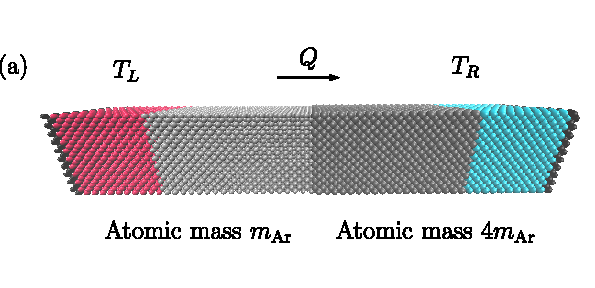
\includegraphics[width=.59\columnwidth]{pics/nemd_fig2a_2.pdf} 
  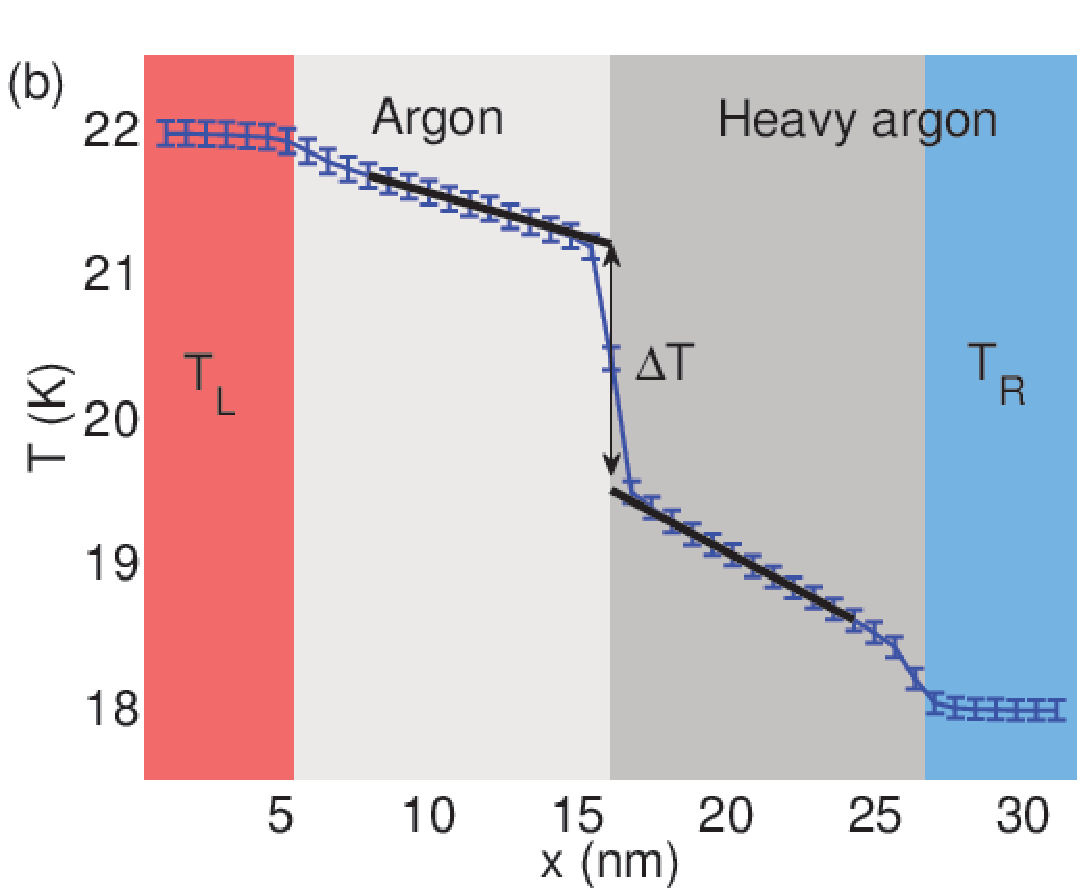
\includegraphics[width=.59\columnwidth]{pics/nemd_fig2b_2.pdf}
  \caption{(a) Simulation geometry used in \citepub{spectral} for investigating the role of anharmonic effects on vibrational energy transfer at mass-mismatched interfaces. (b) Steady-state temperature profile for a specific set of parameters. For details, see \citepub{spectral}.}  
\label{fig:th_spectral_geom}
 \end{center}
\end{figure}


To outline the typical steps involved in a non-equilibrium simulation, consider the example setup of Fig. \ref{fig:th_spectral_geom}(a) used to investigate the anharmonic effects in interfacial heat transfer in \citepub{spectral}. First the whole structure is equilibrated by running a zero-pressure simulation at prescribed temperature using a combination of a Nose-Hoover barostat and thermostat, allowing the structure to conform to zero-stress state. Typical equilibration period consists of a few hundreds of thousands of time steps. After the initial equilibration, the size of the simulation box is fixed, as are atoms located at the left- and right-most unit cells in the system. This prevents atomic sublimation at the free surfaces. Particles in the ''hot'' and ''cold'' regions, illustrated by the red and cyan coloured atoms in Fig. \ref{fig:th_spectral_geom}, are coupled to heat baths at temperatures $T_{\textrm{L}}$ and $T_{\textrm{R}}$. The system is then allowed to reach non-equilibrium steady state by running MD until the temperature profile shown in Fig. \ref{fig:th_spectral_geom}(b) and the heat current flowing through the system fluctuate around constant values. After this initial period, simulation is continued typically for millions of time steps, and the values of the observables of interest are collected from the run. The statistical error in the collected observables can be estimated by using standard methods described, e.g., in \cite{allentildesley}.

% LAMMPS, house-made code

\subsubsection{Spectral heat current analysis}


%This chapter is devoted to the microscopic theory of energy transfer. In Sec. \ref{sec:th_vibtheory}, the theoretical description of atomic vibrations in a lattice is described. 

% In the publications included in this thesis, we have employed molecular dynamics (MD) simulations and Green's function (GF) calculations to model vibrational heat transfer in nanostructures. It is common to both of these methods that one needs to choose how to describe interatomic interactions and the coupling to external heat baths. Before describing MD and GF calculations in Secs. \ref{sec:md} and \ref{sec:gf}, we therefore briefly review the chosen interatomic potentials and the theory of Langevin heat baths below in Secs. \ref{sec:th_interatomicpotential} and \ref{sec:th_langevin}. When discussing the MD method, we also present the recently developed expression for the spectral heat current distribution.

% For electromagnetic energy transfer, we have employed the same Langevin theory as in vibrational heat transfer to describe the microscopic dipolar thermal fluctuations. This theory is presented in Sec. \ref{sec:em_methods}

\iffalse

\section{Vibrational heat transfer}
\label{sec:th_vibtheory}

This section details the theory of vibrational heat transfer in nanoscale. We start in Subsection \ref{sec:th_phonons} by defining the lattice Hamiltonian and define phonons. Various models for interatomic potential energy used in this thesis are listed in Subsection \ref{sec:th_interatomicpotential}. Langevin theory, which is used in all but one publication of this thesis for the theoretical description of thermalization, is detailed in Subsection \ref{sec:th_langevin}.

\subsection{Lattice Hamiltonian and phonons}
\label{sec:th_phonons}
%As discussed in Chap. 1, propagating lattice vibrations carry heat in crystalline solids, and the quanta of such propagating vibrations are called phonons. The theoretical description is based essentially on the equations of motion for the atoms in the solid. Because fully quantum description does not easily allow for accounting for non-linear dynamics, which play an essential role in any system with non-negligible phonon-phonon interactions, the discussion below treats the atomic dynamics classically. 

%\begin{itemize}
% \item The goals of this work
%\end{itemize}
The theoretical description of lattice heat transfer is based on the dynamical equations of motion for the atoms constituting the lattice. The equations of motion are generally dictated by the Hamiltonian \cite{ziman}
\begin{equation}
 \ca{H} = \sum_{i=1}^N \frac{\bb{p}_i^2}{2m_i} + \ca{V}(\bb{r}_1,\dots,\bb{r}_N). \label{eq:th_hamiltonian}
\end{equation}
Here $\br_i$, $\bp_i$, and $m_i$ are the position, momentum and mass of atom $i$, respectively. The total number of atoms (which can also be infinite) is denoted by $N$. The first term of Eq. \eqref{eq:th_hamiltonian} is the total kinetic energy of the atoms and the second term $\ca{V}$ is the interatomic potential energy responsible for the interatomic interactions. The choice of the potential energy function $\ca{V}$ is crucial for an accurate description of the lattice dynamics and, consequently, of energy transfer. Models for $\ca{V}$ used in this work are explained in detail bwlow in Subsection \ref{sec:th_interatomicpotential}.

Applying Hamilton's equations of motion $\dot{\br}_i=\partial H/\partial \bp_i$ and $\dot{\bp}_i=-\partial \ca{H}/\partial \br_i$ \cite{fetter} gives Newton's law
\begin{equation}
 m_i \ddot{\br}_i = \bb{F}_i, \label{eq:th_eom}
\end{equation}
where the force acting on atom $i$ is
\begin{equation}
 \bb{F}_i = - \frac{\partial \ca{V}}{\partial \bb{r}_i}. \label{eq:th_force}
\end{equation}
For given initial conditions $\br_i(0)$ and $\dot{\br}_i(0)$, Eq. \eqref{eq:th_eom} determines the time evolution of atomic trajectories. To model energy transfer, the equations of motion are supplemented by terms accounting for coupling to external heat baths. In this work, we mostly employ Langevin heat baths that turn the equations of motion into stochastic equations and ensure that the long-term atomic trajectories correctly sample the non-equilibrium statistical ensemble. Langevin theory is presented in Sec. \ref{sec:th_langevin}.

Equation \eqref{eq:th_eom} generally describes the motions of atoms and molecules in solid, gas, and liquid systems. In solids, the atoms vibrate close to their equilibrium positions $\br_i^0$ and one can gain more insight into the lattice dynamics by only considering small displacements from the equilibrium. The positions $\br_i^0$ are defined by the condition of zero force:
\begin{equation}
 \left. \frac{\partial \ca{V}}{\partial \br_i} \right|_{\br_j=\br_j^0 \quad \forall j} = 0. \label{eq:th_zeroforce}
\end{equation}
Assuming that the atoms remain close to the equilibrium positions, one can expand the potential energy in Taylor series in terms of the displacements $\bu_i=\br_i-\br_i^0$:
\begin{equation}
 \ca{V} = \ca{V}_0 + \frac{1}{2} \sum_{i,j} \sum_{\alpha,\beta} u_i^{\alpha} K_{ij}^{\alpha \beta} u_j^{\beta}  + \ca{O}(u^3). \label{eq:th_V_taylor}
\end{equation}
Here the Cartesian coordinate directions $\alpha,\beta \in \{x,y,z\}$ have been written explicitly for clarity and the second-order term is proportional to the ''force constant''
\begin{equation}
 K_{ij}^{\alpha\beta} = \left. \frac{\partial^2 \ca{V}}{\partial u_i^{\alpha} \partial u_j^{\beta}} \right|_{\bu=\mathbf{0}}. \label{eq:th_K_def}
\end{equation}
The first-order derivative term in \eqref{eq:th_V_taylor} vanished based on Eq. \eqref{eq:th_zeroforce} and the last term is of third order in displacements.

In the case that the third-order term can be neglected, employing Eq. \eqref{eq:th_V_taylor} in the equation of motion \eqref{eq:th_eom} gives the system of linear equations
\begin{equation}
 m_i \ddot{u}_i^{\alpha} = - \sum_j \sum_{\beta} K_{ij}^{\alpha\beta} u_j^{\beta}.
\end{equation}
Following standard eigenmode theory \cite{fetter}, the eigenmodes of the system can be found by diagonalizing the matrix $D_{ij}^{\alpha\beta} = (m_i\omega^2 \delta_{ij}\delta
^{\alpha\beta}-K_{ij}^{\alpha\beta})$. In a periodically repeating crystal, the eigenmodes can be labeled by the wavevectors $\bb{q}$ belonging to the first Brillouin zone \cite{ziman} and the branch $p \in \{1,\dots,3N_{\textrm{cell}}\}$, where $N_{\textrm{cell}}$ is the number of atoms in the unit cell. The eigenmodes are called phonon modes, while phonons are the discrete quanta of eigenmode occupation. The eigenfrequencies $\omega(\bb{q},p)$ form the phonon bandstructure, specifying the relation between the wavevectors and frequencies supporting propagating phonon modes. As an example, Fig. \ref{fig:th_nika} shows the phonon bandstructure of graphene, a single monolayer of graphite.

\begin{figure}
\begin{center}
 \includegraphics[width=8.6cm]{pics/nika09_fig3.pdf}
 \caption{Phonon bandstructure of graphene, calculated using the valence force field method \cite{nika09}. The two-dimensional bandstructure is plotted along one-dimensional lines between special points in graphene reciprocal lattice, denoted by $\Gamma$, $M$ and $K$. Because graphene has two atoms per unit cell, there are altogether six phonon branches. The three branches that have vanishing frequencies at the $\Gamma$ point are called longitudinal acoustic (LA), transverse acoustic (TA) and out-of-plane acoustic (ZA). The optical modes LO, TO and ZO are labeled similarly. Reprinted with permission from Ref. \cite{nika09}.}
\label{fig:th_nika}
\end{center}
\end{figure} 

When the anharmonic part in Eq. \eqref{eq:th_V_taylor} is neglected, the phonon eigenmodes are exact eigenmodes of the system and cannot dissipate their energy, giving rise to infinite thermal conductivity \cite{ziman}. The anharmonic terms give rise to phonon-phonon scattering \cite{ziman}, which is the primary phonon decay mechanism in crystalline solids at high temperatures. In Publications \cp{fpu}, \cp{fpu2}, \cp{spectral}, \cp{cnt}, and \cp{twinning}, we have employed classical molecular dynamics simulations fully accounting for anharmonic scattering. In \citepub{gf}, anharmonic effects are mimicked by the self-consistent heat bath model \cite{bolsterli70}, allowing for the inclusion of quantum statistics as well. These methods are explained in more detail below in Chap. XXX.

\subsection{Models for interatomic potential energy}
\label{sec:th_interatomicpotential}

%Typically, the analytical form of the interatomic potential is inferred from quantum-mechanical calculation and the free parameters are fitted to reproduce experimentally known quantities such as the lattice constant, bulk modulus, atomization energy, and so on. For this reason, the interatomic potentials are often called semi-empirical. In chemistry, the term force field is used instead of interatomic potential.

As mentioned in Sec. \ref{sec:intro_vibtheory}, a crucial physical aspect of correctly describing the lattice dynamics and, therefore, vibrational energy transfer is the choice of interatomic potential energy function $\ca{V}$. In general, the interatomic potential consists of pair potential terms and many-body terms. 
%, which we assume to only consist of the three-body terms $V^{(3)}(\bb{r}_i,\bb{r}_j,\bb{r}_k)$:
%\begin{equation}
% U(\bb{x}) = \frac{1}{2}  \sum_{ i,j } V^{(2)}(|\bb{r}_{i}-\bb{r}_j|) + \frac{1}{6} \sum_{i,j,k} V^{(3)}(\bb{r}_i,\bb{r}_j,\bb{r}_k)
%\end{equation}
A very simple example of a pure pair-potential is the Fermi-Pasta-Ulam (FPU) potential used by Fermi, Pasta, and Ulam to investigate the minimal necessary conditions for thermalization in one-dimensional system. In the FPU model, atoms with displacement $u_i$ from the equilibrium position are assumed to be connected to their nearest neighbors by anharmonic springs with the pair-wise energy of the form
\begin{equation}
  V_{ij}^{\textrm{FPU}} = \frac{1}{2} k (u_i-u_j)^2 + \frac{\alpha}{3} (u_i-u_j)^3+ \frac{\beta}{4} (u_i-u_j)^4, \label{eq:th_fpu}
\end{equation}
which is referred to as the FPU potential. The FPU potential can be considered to arise from the Taylor expansion of a more realistic potential (such as LJ). The models for $\beta=0$ and $\alpha=0$ are known as $\alpha$-FPU and $\beta$-FPU, respectively, and both have been employed extensively in investigating thermalization and thermal conduction in low-dimensional systems \cite{}. In Publications \cp{fpu} and \cp{fpu2}, the $\beta$-FPU potential was used to model the anharmonic interactions in a square lattice. In Publication \cp{gf}, the anharmonic interactions were mimicked by the coupling to self-consistent heat baths (see Sec. \ref{sec:gf}), and only the harmonic term of Eq. \eqref{eq:th_fpu} was included ($\alpha=\beta=0$).

Another very common pair-potential is the Lennard-Jones (LJ) potential \cite{allentildesley}
\begin{equation}
 V_{ij}^{\textrm{LJ}}(r_{ij}) = 4\varepsilon \left[\left( \frac{\sigma}{r_{ij}}\right)^{12}-\left( \frac{\sigma}{r_{ij}}\right)^6  \right],
\end{equation}
where $\varepsilon$ is the interaction energy, $\sigma$ determines the equilibrium distance $r_0$ of atoms ($r_0=2^{1/6}\sigma$ for two particles), and $r_{ij}$ is the interparticle distance. The repulsive term $(\sigma/r_{ij})^{12}$ models the strong atomic repulsion at short distances, arising from the overlapping of electron clouds. The attractive term $-(\sigma/r_{ij})^{6}$ accounts for the weak van der Waals attraction at large distances, arising from the interaction of the fluctuating dipole moments due to, e.g., electron polarization. The LJ potential accurately describes interatomic interactions between noble gas atoms such as argon and, thanks to its simple form, it is also often used to investigate the qualitative features of heat transfer in solids \cite{}. The LJ potential was used in Publication \cp{spectral} to model the interatomic interactions in investigating the spectral conductance between mass-mismatched solids arranged in a face-centered cubic lattice. %Because the LJ interaction does not account for the local environment, however, the LJ potential cannot describe, e.g., covalent bonding. %It is used a constituent in more complicated potentials to describe the van der Waals attractions. Due to its simple form, it is also often used 


Pure pair-potentials such as the Lennard-Jones potential cannot describe, e.g., covalent bonding, where the strength of local bonding is strongly influenced by the environment. Therefore, a more sophisticated potential is needed to model, for example, carbon materials. A typical example of a many-body potential is the Tersoff potential \cite{tersoff88b}
\begin{equation}
 V_{ij}(r_{ij}) = f_C(r_{ij}) \left[A e^{-\lambda_1 r_{ij}} - B b_{ij} e^{-\lambda_2 r_{ij}}) \right],
\end{equation}
where the taper function 
\begin{equation}
 f_C ( r) = \left\{ \begin{array}{ll}
                     1 & \textrm{for } r<R-D,\\
		     \frac{1}{2}-\frac{1}{2}\sin\left(\frac{\pi}{2}\frac{r-R}{D} \right) & \textrm{for } R-D < r < R+D, \\
		     0 & \textrm{for } r>R+D
                    \end{array}
 \right.
\end{equation}
gradually turns off the pair-wise interaction between $r_{ij}=R-D$ and $r_{ij}=R+D$. The strength of interatomic attraction is controlled by the coefficient
\begin{equation}
 b_{ij} = \left( 1+\beta^n \zeta_{ij}^n \right)^{-1/(2n)},
\end{equation}
where the dependence on the local environment appears in the definition 
\begin{equation}
 \zeta_{ij} = \sum_{k\neq i,j} f_C(r_{ik}) g(\Theta_{ijk}) \exp\left[\lambda_3^3(r_{ij}-r_{ik})^3 \right] .
\end{equation}
Here $\Theta_{ijk}$ is the angle between bonds $ij$ and $ik$. The angle function is defined as 
\begin{equation}
 g(\Theta) = 1 + \frac{c^2}{d^2} - \frac{c^2}{d^2 + (\cos \Theta-\cos \Theta_0)^2}
\end{equation}
The parameters $R$, $D$, $A$, $\lambda_1$, $B$, $\lambda_2$, $\beta$, $n$, $\lambda_3$, $c$, $d$, and $\Theta_0$ depend on the material under study. The Tersoff parameters for carbon systems were originally fit to the experimentally known cohesive energies of various carbon systems and the lattice constant and bulk modulus of diamond \cite{tersoff88a}. Recently, Lindsay and Broido \cite{lindsay10} suggested an improved set of parameters found by giving more weight to matching the experimentally measured phonon dispersion for graphite. This optimized Tersoff potential was used in Publication \cp{cnt} for carbon nanotubes. In \citepub{twinning}, many-body Stillinger-Weber potential \cite{stillinger85} was used to model interactions between Si atoms constituting Si nanowire. 


\subsection{Langevin theory} 
\label{sec:th_langevin}
The equations of motion \eqref{eq:th_eom} only describe the interactions between the constituents of the system under study. To enable steady-state energy transfer, some of the degrees of freedom must be coupled to external heat baths acting as heat sources and sinks. Because Langevin heat baths are employed in all but one publication included in this thesis, we briefly review the Langevin theory.

In Langevin theory, the particle coupled to the bath is imagined to interact with a collection of harmonic oscillators at a prescribed temperature. The bath degrees of freedom are ''integrated out'' so that their interaction with the system under study is described effectively by the Langevin forces \cite{weiss}. The general Langevin equation obtained through such a procedure reads \cite{dhar06}
\begin{equation}
 m\ddot{\bu}_i(t) =  \bb{F}_i(t) - \int_{0}^{\infty}dt' \Sigma_i(t') \bb{u}_i(t-t') + \xi_i(t), \label{eq:th_eom_langevin}
\end{equation}
where, for the simplicity of discussion, we assume that the baths are spatially uncorrelated so that the bath self-energy $\Sigma_i$ is spatially local. The self-energy describes the dynamical interactions and damping induced by the coupling to the heat bath oscillators. The force $\bb{F}_i$ is due to interactions with particles not in the reservoir and the auto-correlation function of the random force $\xi_i$ is related to the damping self-energy $\Sigma_i(t)$ and bath temperature $T_i$ through the fluctuation-dissipation theorem (FDT) \cite{dhar06}
\begin{equation}
 \langle \xi_i(t)\xi_i(t') ^T\rangle = \int_{-\infty}^{\infty} \frac{d\omega}{2\pi} e^{-i\omega(t-t')} \hbar \Gamma_i(\omega) \left[f_B(\omega,T_i)+\frac{1}{2}\right] \bb{I}_{3\times3}. \label{eq:th_xixit}
\end{equation}
Here $\Gamma_i(\omega)=-2\textrm{Im}[\Sigma_i(\omega)]$ is called the bath coupling function \cite{dhar06}. The quantum statistics appear through the Bose-Einstein occupation function $f_B(\omega,T)=\left\{\exp[\hbar\omega/(k_BT)]-1 \right\}^{-1}$. By Fourier transforming with respect to $t$ and $t'$ separately, Eq. \eqref{eq:th_xixit} can be written in the form useful for calculations:
\begin{equation}
  \langle\tilde  \xi_i(\omega)\tilde \xi_i(\omega')^T \rangle = 2\pi\hbar\delta(\omega+\omega') \Gamma_i(\omega) \left[f_B(\omega,T_i)+\frac{1}{2} \right] \bb{I}_{3\times3}. \label{eq:th_xixiom}
\end{equation}

To simulate Langevin dynamics in a MD simulation, it is useful to write the integral term appearing in the Langevin equation in terms of the velocity $\dot{u}(t)$. To achieve this, one can integrate in Eq. \eqref{eq:th_eom_langevin} partially to get
\begin{equation}
 m\ddot{\bu}_i(t) =  \bb{F}_i(t) - \int_{0}^{\infty}dt' M(t')\dot{\bb{u}}_i(t-t') + \xi_i(t). \label{eq:th_langevin_Mt}
\end{equation}
The boundary terms appearing in the partial integration are assumed to vanish because we (i) define the integral function $M(t)=-\int_t^{\infty} dt' \Sigma(t')$ of $\Sigma(t)$ for positive $t$ so that $M(t\to \infty)=0$ and (ii) the term proportional to $M(0)u(t)$ can be absorbed to the external force $F[u(t)]$ or eliminated by re-defining the displacements \cite{weiss}. The classical Langevin equation is obtained by choosing a very rapidly decaying $M(t)$ and taking the limit of vanishing decay time, allowing for arriving at the classic Langevin equation \cite{zwanzig}
\begin{equation}
 m\ddot{\bu}_i(t) =  \bb{F}_i(t) - m\gamma \dot{\bu}_i(t) + \xi_i(t). \label{eq:th_ohmic}
\end{equation}
This form of damping, proportional to the instantaneous velocity $\dot{\bu}(t)$ and the friction constant $\gamma$, is called Ohmic damping due to its analogue with a resistor in an electrical circuit \cite{weiss}. This form can be shown to give rise to a frequency-independent phonon relaxation time $\tau=1/\gamma$ \cite{li09jap}. The corresponding FDT \eqref{eq:th_xixiom} for the force variance is, for Ohmic damping,
\begin{equation}
 \langle \tilde \xi_i(\omega) \tilde \xi_i(\omega')^T \rangle = 4\pi \delta(\omega+\omega') \hbar \omega \gamma \left[f_B(\omega,T_i)+ \frac{1}{2} \right] \bb{I}_{3\times 3}. \label{eq:th_xixiom_ohmic_qm}
\end{equation}
In the classical high-temperature limit relevant for classical molecular dynamics, one gets the classical FDT \cite{zwanzig}
\begin{equation}
 \langle \xi_i(t) \xi_i(t')^T\rangle=2\gamma k_B T_i \delta(t-t') \bb{I}_{3\times 3}. \label{eq:th_corr_ohmic} 
\end{equation}

In this thesis, we employ the Ohmic damping of Eq. \eqref{eq:th_ohmic} due to its simplicity. In Publications \cp{fpu}, \cp{fpu2}, \cp{spectral}, and \cp{cnt}, Ohmic Langevin heat baths are used as hot and cold heat baths in the molecular dynamics simulation. In accordance with the classical dynamics, the classical FDT \eqref{eq:th_corr_ohmic} is employed for force variance. \citepub{twinning} employs classical Nose-Hoover heat baths \cite{hoover85} instead of Langevin heat baths. 

In Publication \cp{gf}, Langevin heat baths act not only as external thermal reservoirs but also as pathways for phonon creation and annihilation inside the system under study. This is the self-consistent heat bath model \cite{bolsterli70} explained in detail in Sec. \ref{sec:th_selfconsistentbaths}. In Publication \cp{dipole}, Langevin baths are used to model thermal fluctuations and dissipation of dipole moments. Because the equations of motion are linear in the two latter cases, we can also account for quantum statistics by using the quantum fluctuation-dissipation theorem \eqref{eq:th_xixiom_ohmic_qm}.


\section{Electromagnetic energy transfer}

% \subsection{Theoretical background}

\label{sec:theory_emtheory}

\subsection{Field due to an oscillating dipole}

The theoretical description of electromagnetic energy transfer between oscillating dipoles is based on Maxwell equations \cite{novotny}. In the non-magnetic materials with no free charges that are considered in this work, the electromagnetic fields arise from the fluctuating electric polarization fields inside the bodies, and the Maxwell equations for the electric field $\bE(\br,t)$ and magnetic field $\bb{H}(\br,t)$ read \cite{novotny}
\begin{subequations}
\begin{align}
  \nabla \times \bE(\br,t) &= - \mu_0 \frac{\partial \bb{H}(\br,t)}{\partial t}, \label{eq:th_maxwell1} \\
  \nabla \times \bb{H}(\br,t) &= \varepsilon_0 \frac{\partial \bb{E}(\br,t)}{\partial t} + \frac{\partial \bb{P}(\br,t)}{\partial t}, \label{eq:th_maxwell2} \\
   \nabla \cdot \bb{H}(\br,t) &= 0, \\
   \nabla \cdot \bb{E}(\br,t) &= 0.
\end{align}
\end{subequations}
Equation \eqref{eq:th_maxwell2} shows that a temporal change in the polarization density $\bb{P}(\br,t)$ gives rise to a magnetic field, which in turn induces an electric field according to Eq. \eqref{eq:th_maxwell1}. The induced electromagnetic field carries energy flux, whose magnitude and direction are given by the Poynting vector $\bb{S}(\br,t)=\bb{E}(\br,t)\times \bb{H}(\br,t)$ \cite{novotny}.

To determine the amount of energy radiated by a fluctuating dipole, one needs to solve for the electric and magnetic fields emitted by the dipole current density distribution $\bb{j}(\br',t)=\partial \bb{P}(\br,t)/\partial t$. As shown in detail in Ref. \cite{novotny}, the electric field is given in frequency-domain by 
\begin{equation}
 \tilde \bE(\br,\omega) = \tilde \bE_0(\br,\omega) + i \omega \mu_0 \int_V d\mathbf{r}' \mathbb{G}(\br,\br';\omega) \tilde{\bb{j}}(\br',\omega). \label{eq:th_Etilde}
\end{equation}
Here $\tilde{\bE}_0(\br,\omega)$ is the electric field arising from sources other than the oscillating dipoles, volume $V$ encloses the dipoles and $\mathbb{G}(\br,\br';\omega)$ is the electromagnetic Green's dyadic found by solving the Helmholtz equation \cite{novotny}
 \begin{equation}
 \nabla \times \nabla \times \gem(\bb{r},\br';\omega) - (\omega^2/c^2) \epsenv(\br,\omega)\gem(\bb{r},\br';\omega)  =  \delta(\bb{r}-\br')\unitdyadic. \label{eq:intro_gemdef}
\end{equation}
Here $c$ is the speed of light and $\epsenv(\br,\omega)$ is the relative dielectric constant of the environment. The Green's dyadic can generally be decomposed into the free-space and scattered parts as
\begin{equation}
 \mathbb{G}(\br,\br';\omega ) = \mathbb{G}_0(\br,\br';\omega ) + \mathbb{G}_s(\br,\br';\omega ). \label{eq:th_G_decomp}
\end{equation}
The first term, which corresponds to the field radiated by the dipole in absence of any scattering events, is \cite{novotny}
\begin{equation}
 \mathbb{G}_0(\br,\br';\omega) = \left[\mathbf{I}_{3\times 3} + \frac{1}{k_0^2} \nabla \nabla \right] \frac{e^{ik_0|\br-\br'|}}{4\pi|\br-\br'|}.
\end{equation}
Here $k_0=\omega/c$ is the wavevector in vacuum and $\mathbf{I}_{3\times 3}$ is the $3\times 3$ identity matrix. The second term $\mathbb{G}_s(\br,\br';\omega)$ accounts for the scattering of the emitted field by the inhomogeneities in the environment such as reflecting walls. The decomposition \eqref{eq:th_G_decomp} is useful, because the two terms behave differently for $\br\to \br'$: the dyadic $\mathbb{G}_0$ diverges for $\br\to \br'$, but the scattering part $\mathbb{G}_s$ is smooth \cite{novotny}. Having the expression \eqref{eq:th_Etilde} for the electric field, the magnetic field $\tilde{\bb{H}}(\br,\omega)$ can be solved from the first Maxwell equation \eqref{eq:th_maxwell1}, and one can calculate the Poynting vector $\bb{S}$.

\subsection{Fluctuational electrodynamics}

To calculate the energy transfer between bodies, we need an equation specifying the relation between the fluctuations in dipole moments and the material's optical properties and temperature. The traditional approach is the fluctuational electrodynamics (FED) theory pioneered by Rytov \cite{rytov} and Lifshitz \cite{lifshitz55}. The core of FED is the fluctuation-dissipation relation \cite{novotny,agarwal75_1}
\begin{equation}
 \langle \tilde{\bp}(\omega)\tilde{\bp}(\omega')^T\rangle = 4\pi \hbar \delta(\omega+\omega')  \textrm{Im}[\alpha(\omega)] \left[f_B(\omega,T)+\frac{1}{2} \right], \label{eq:th_fed_fdt}
\end{equation}
which is used to relate the stochastic fluctuations in the local dipole moment $\tilde{\bp}(\omega)$ (which is the local dipole density integrated over a small volume) to the imaginary part of the dipole polarizability dyadic $\alpha(\omega)$ and dipole temperature $T$. 

While Eq. \eqref{eq:th_fed_fdt} has been used to successfully calculate energy transfer rates in various situations \cite{}, there are two arguments supporting a more microscopic approach. First, because FED relies on an effective medium property, the local polarizability, applying the theory to very small systems requires great care. It was noted only recently by Manjavacas and Abajo de Carc\'ia \cite{manjavacas12} that the fluctuation-dissipation relation connecting the polarization to the polarizability must be modified when local radiative corrections become important to ensure that non-absorbing particles do not emit thermal radiation. Starting from a more microscopic theory would make it possible to avoid resorting to effective medium parameters in the formulation. Second, one can envision  when the optical phonons responsible for electromagnetic radiation cannot be considered to be decoupled from the acoustic phonons responsible for ''phonon radiation''. In such cases, it is necessary to describe the full lattice dynamics and its coupling to the electromagnetic field microscopically. 

In Publication \cp{dipole}, we developed such a microscopic generalization of fluctuational electrodynamics, basing the description of thermal fluctuations on writing quantum Langevin equations for the microscopic dipole oscillations. By starting from the microscopic equations of motion, we could straightforwardly derive expressions for heat transfer rates between dipoles in an inhomogeneous environment in full analogy to the phononic case treated in \citepub{gf}, directly accounting also for local radiative corrections. The theory is presented in Sec. \ref{sec:em_methods}.


\section{Electron transport}

\subsection{Tight-binding model}




% The thermal background field $\Eenvhat$ has zero average $\langle \Eenvhat \rangle=0$ and its symmetrized autocorrelation function satisfies the fluctuation-dissipation relation 


% \subsection{Introduction to Green's functions}
% 
% \label{sec:gf_linear}
% Green's function method is based on inverting the ''equation of motion operator'', which we will discuss later. For a general non-homogenous equation of the form
% \begin{equation}
%  \mathcal{L} f = g,
% \end{equation}
% where $\mathcal{L}$ is a linear operator and $g$ is the source function, symbolic solution in terms of the Green's function $\mathcal{G}$ is
% \begin{equation}
%  f = \mathcal{G} g.
% \end{equation}
% The Green's function $\mathcal{G}$ is defined as the inverse of $\mathcal{L}$:
% \begin{equation}
%  \mathcal{L} \mathcal{G} = I,
% \end{equation}
% where $I$ is the identity operator. Since $\mathcal{L}$ is linear, solution for 
% \begin{equation}
%  \mathcal{L} f = g_1 + g_2
% \end{equation}
% is the sum of solutions
% \begin{equation}
%  f = \mathcal{G}g_1 + \mathcal{G} g_2.
% \end{equation}
% Calculating $\mathcal{G}$ for a given $\mathcal{L}$ determines, therefore, the solution for any source function $g$. 
% 
% 
% 
% \subsection{Quantum mechanical Green's functions}
% 
% For completeness, we also briefly discuss the Green's functions that appear in the quantum-mechanical many-body problem. These functions are directly defined as statistical averages of different correlation functions and, at first sight, bear no resemblance to the Green's function discussed in Sec. \ref{sec:gf_linear}. The most used two-particle Green's functions are \cite{wang08}
%  \begin{alignat}{2}
%    G^R(t,t') &= -i\theta(t-t') \langle [\bb{u}(t), \bb{u}(t')^T] \rangle \\
%    G^A(t,t') &= i\theta(t'-t) \langle [\bb{u}(t), \bb{u}(t')^T] \rangle\\
%    G^>(t,t') &= -i\langle \bb{u}(t) \bb{u}(t')^T \rangle\\
%    G^<(t,t') &= -i\langle \bb{u}(t') \bb{u}(t)^T \rangle^T	 \\
%    G^t(t,t') &= \theta(t-t') G^>(t,t') + \theta(t'-t) G^<(t,t') \\
%    G^{\bar t}(t,t') &=\theta(t'-t) G^>(t,t') + \theta(t-t') G^<(t,t')  ,
%  \end{alignat}
% which are called the retarded, advanced, greater, lesser, time-ordered and anti-time-ordered Green's functions, respectively. The operators appearing inside the expectation values are written in Heisenberg picture. Out of the six Green's functions, only three are linearly independent and, in steady-state, the number of independent functions is reduced to two. In equilibrium, one of the Green's functions determines the others, and typically $G^R$ is considered. Note that $G^R$ satisfies
% \begin{alignat}{2}
%  \partial_t G^R(t,t')  &= -i \delta(t-t')  \langle [\bb{u}(t), \bb{u}(t')^T] \rangle -i \theta(t-t') \langle [\dot{\bb{u}}(t),\bb{u}(t')^T ] \rangle \\
%   &= -i \theta(t-t') \langle [\bb{p}(t),\bb{u}(t') ]^T \rangle
% \end{alignat}
% and
% \begin{alignat}{2}
%  \partial_t^2 G^R(t,t') &= - i \delta(t-t') \langle [\bb{p}(t),\bb{u}(t') ]^T \rangle - i \theta(t-t') \langle [\dot{\bb{p}}(t),\bb{u}(t')^T] \rangle \\
%   &= - \delta(t-t')\bb{I}  - i \theta(t-t') \langle [\dot{\bb{p}}(t),\bb{u}(t')^T] \rangle .
% \end{alignat}
% For a quadratic Hamiltonian 
% \begin{equation}
%  \mathcal{H} = \frac{\bb{p}^2}{2} + \frac{1}{2} \bb{u}^T \bb{K} \bb{u},
% \end{equation}
% the Heisenberg equation of motion for $\bb{p}(t)$ is 
% \begin{equation}
%  \dot{\bb{p}}(t) = - \bb{K} \bb{u}(t),
%  \label{eq:dotpt}
% \end{equation}
% so 
% \begin{equation}
%  \partial_t^2 G^R_{ij} (t,t') = - \delta(t-t') \delta_{ij} - K_{ik} G^R_{kj}(t,t').
% \end{equation}
% Fourier transformation then gives the familiar Green's function
% \begin{equation}
%  G^R(\omega) = [(\omega+i\eta)^2-\bb{K}]^{-1}
% \end{equation}
% from the last section. This short calculation justifies the name Green's function. Note that for an interacting system, Eq. \eqref{eq:dotpt} would not be valid and the hiearchy of equations of motion would not close.
% 
% The usefulness of Green's functions in the statistical mechanics of quantum-mechanical systems lies in the facts that (1) they can be used to calculate all thermodynamic observables \cite{negele}, and (2) they allow an easy and intuitive perturbative expansion that can be represented as Feynman diagrams \cite{negele,fetter2}. At zero and non-zero temperature, the diagrammatic expansion in terms of the interaction parameter is carried out for the time-ordered Green's function and the Matsubara Green's function, respectively. Methods such as functional renormalization group \cite{metzner12,saaskilahti11} can be applied to sum a subset of diagrams up to an infinite order in a controlled manner.
% 
% In the context of non-equilibrium transport problem, Meir and Wingreen showed that the electronic current through an \textit{interacting} system can be written in terms of $A(\omega)$, the spectral function of the system. Corresponding formula for phonon transport through an anharmonic system was derived by Wang \cite{wang06} and Mingo \cite{mingo06}, and the formula reads for, say, the current flowing to the left lead
% \begin{equation}
%  I = \int \frac{d\omega}{2\pi} \omega \textrm{Tr}\left[G^R(\omega) \Sigma^<(\omega) + G^<(\omega) \Sigma^A(\omega) \right],
% \end{equation}
% where $\Sigma^<$ and $\Sigma^A$ are the lesser and advanced self-energies of the left lead. To calculate the Green's functions and self-energies perturbatively, the perturbation expansion is done for the more general Keldysh Green's function
% \begin{equation}
%  G (\tau,\tau') = -i \langle \mathcal{T}_{\tau} u(\tau) u(\tau') \rangle.
% \end{equation}
% Time variable $\tau$ lies on the Keldysh contour, which runs from $-\infty$ to $\infty$ slightly above the real axis and back to $-\infty$ slightly below the real axis \cite{jauho}.



%\begin{itemize}
% \item Definition of polarizability, optical theorem
% \item Coupling of optical and acoustic degrees of freedom
%\end{itemize}


\iffalse
\begin{equation}
 \left\langle \tilde{j}^{\alpha}(\br,\omega)\tilde{j}^{\beta}(\br',\omega') \right\rangle = 2\pi \delta(\omega+\omega') \times 2\omega \varepsilon_0 \textrm{Im}[\varepsilon(\br,\br';\omega)] \hbar \omega \left[f_B(\omega,T)+\frac{1}{2} \right]
\end{equation}
\fi
%\begin{itemize}
% \item Maxwell equations
% \item Fluctuational electrodynamics
% \item Electromagnetic Green's function
%\end{itemize}
% Loomis and Maris 94: We present a macroscopic, phenomenological theory for the heat flow between two material half-spaces of differing temperatures whose surfaces are separated by a gap of width l. Our calculation parallels Liftshitz's calculation of the van der Waals force between two dielectric slabs. For l sufficiently small, the heat flow is enhanced by a contribution from evanescent waves, and in the limit of a very small gap varies as l^{-2}.




\iffalse
Usually, the bath self-energy $\Sigma(\omega)$ is given to specify the coupling with the bath. Therefore, it is useful to derive an expression relating the bath self-energy to $M(t)$. This process is complicated by the fact that because $M(t)$ does not vanish at negative infinity, one cannot use the Fourier transform of $M(t)$ in the process. However, because only the values of $M(t)$ for $t>0$ play a role in Eq. \eqref{}, one can introduce a step-function in the integral and substitute the convenient definition $M^e(t)=\Theta(t)M(t)+\Theta(-t)M(-t)$:
\begin{equation}
 m\ddot{u}(t) =  F[u(t)] - \int_{-\infty}^{\infty}dt'\Theta(t') M^e(t')\dot{u}(t-t') + \xi(t).
\end{equation}
One can then easily show that the Fourier transform of $M^e(t)$ is related to the bath self-energy $\Sigma(\omega)$ through the coupling function $\Gamma(\omega)=-2\textrm{Im}[\Sigma(\omega)]$:
\begin{equation}
 \hat M^e(\omega) = \frac{\Gamma(\omega)}{\omega}. \label{eq:th_langevin_Mt}
\end{equation}
In cases where the exact spectral properties of the bath do not matter, the simplest choice for the bath self-energy is
\begin{equation}
 \Sigma(\omega) = -i\gamma \omega \Theta(\omega_c-|\omega|),
\end{equation}
where $\omega_c$ is the cut-off frequency for the bath modes. Equation \eqref{eq:th_langevin_Me} then gives
\begin{equation}
 \hat M^e(\omega) = 2\gamma \Theta(\omega_c-|\omega|), 
\end{equation}
so the friction kernel $M^e(t)$ is 
\begin{equation}
 M^e(t) = 2 \gamma \delta_{\omega_c}(t),
\end{equation}
where 
\begin{equation}
 \delta_{\omega_c} (t) = \frac{1}{\pi} \frac{\sin \omega_c t}{t}. \label{eq:th_langevin_deltat}
\end{equation}
For $\omega_c\to \infty$, Eq. \eqref{eq:th_langevin_deltat} tends to the Dirac Delta function and the friction term in the generalized Langevin equation reduces to the classic Langevin equation 
\begin{equation}
  m\ddot{u} = {F}[{u}(t)] -m \gamma \dot{{u}} + \xi(t). 
\end{equation}
\fi
\iffalse

\subsection{Background}
In his seminal work on the theory of Brownian motion, Paul Langevin added stochastic force terms in the equation of motion to model the essentially random collisions of a particle with the molecules of the surrounding fluid. The additional force consists of two terms, the deterministic damping force proportional to the friction coefficient $\gamma$ and the stochastic force $\xi$:
\begin{equation}
 m \ddot{x} = {F}[{x}(t)] -m \gamma \dot{{x}} + \xi(t). \label{eq:langevin_eq}
\end{equation}
Here ${x}(t)$ is the particle position, $m$ the mass and ${F}[{x}(t)]$ is the force due to particles other than the solvent. For simplicity, we have written the one-dimensional form of the equation. In Langevin theory, the collisions with the solvent (represented by the stochastic force $\xi$) are assumed to average to zero force ($\langle \xi \rangle=0$) and to be temporally uncorrelated: $\langle \xi(t) \xi(t')^T\rangle \propto \delta(t-t')$. To calculate the constant of proportionality in the variance, one can calculate the expectation value of $\langle v^2\rangle$ for $t \to \infty$ to show that the classical equipartition $ m \langle \bb{v}^2 \rangle = k_BT$ only holds if the stochastic force and friction force are related by the relation
\begin{equation}
 \langle \xi(t) \xi(t')\rangle=2\gamma T \delta(t-t'). \label{eq:corr_ohmic} %\mathbf{I}_{3\times 3}
\end{equation}
This is the fluctuation-dissipation relation connecting the magnitude of fluctuations $\xi$ to the dissipation constant $\gamma$. The damping term of Eq. \eqref{eq:langevin_eq} is often referred to as Ohmic damping due to its correspondence with an Ohmic resistor in circuit theory \cite{weiss}.

In this example, the molecules of the solvent act as a thermal reservoir at temperature $T$. For any given initial velocity of the particle, the particle will drift toward thermal equilibrium with the reservoir and eventually achieve it. Building on this idea, Langevin forces are traditionally used in simulations to thermostat the system to a given temperature \cite{}. This allows one to either (i) simulate canonical ensemble at given temperature, (ii) push the system into thermal non-equilibrium by coupling atoms to Langevin thermostats at different temperatures, or (iii) to simulate dissipative and fluctuative processes driving the system to local equilibrium by Langevin thermostats at position-dependent temperatures.
\fi
\iffalse
\section{Langevin bath in simulations}

Langevin bath is typically used for three different tasks. In the first case, Langevin bath is used to simulate canonical ensemble (thermal equilibrium) by coupling all atoms to a bath at single temperaure $T$. In this case, the coupling constant $\gamma$ to the baths should typically be chosen small enough so that the coupling does not disturb the natural vibrational dynamics in the system. If the coupling is too small, however, the energy exchange with the bath is so slow that very long simulation runs are required to properly sample the available phase space.

In the second case, multiple baths at different temperatures are used to push the system into non-equilibrium. In this case, the baths act as heat sources and sinks, and the coupling constant $\gamma$ effectively determines the contact resistance with the reservoirs. While large $\gamma$ generally decreases the contact resistance to the reservoirs, it also increases the acoustic mismatch between thermalized and unthermalized atoms. Therefore, it should be carefully checked that the obtained results (such as thermal resistance) are not sensitive to the exact value of $\gamma$.

Finally, coupling to the Langevin bath can describe \textit{internal} processes driving the system into (local) thermal equilibrium. For example, the complicated phonon-phonon interactions giving rise to phonon creation and annihilation can be described in an effective manner by the fluctuating and dissipative Langevin forces, respectively. The resulting linearization of the equations of motion allows for solving the equations of motion directly in terms of the Green's function. To ensure current conservation, it is necessary to determine the bath temperatures self-consistently so that phonon creation and annihilation are balanced. This is the self-consistent heat bath model.
\fi

\iffalse
\subsection{General Langevin equation}

The original Langevin equation with the classical fluctuation-dissipation relation is typically used in molecular dynamics simulations due to its simplicity. In cases when the spectral properties of the coupling to the bath matter (for example to minimize the contact resistance between the bath and the system) or if quantum statistics must be accounted for, one must turn to the general Langevin theory \cite{weiss}.

In general Langevin theory, the reservoir is modeled as a collection of harmonic oscillators. The bath degrees of freedom are ''integrated out'' so that their interaction with the system under study is described effectively by the Langevin forces. In general, the friction and force then have temporal correlations and the Ohmic damping of Eq. \eqref{eq:langevin_eq} and Markovian force [Eq. \eqref{eq:corr_ohmic}] are replaced by more complicated expressions \cite{weiss}. The general Langevin equation reads \cite{dhar06}
\begin{equation}
 m\ddot{u}(t) =  F[u(t)] - \int_{0}^{\infty}dt' \Sigma(t') {u}(t-t') + \xi(t),
\end{equation}
where the auto-correlation function of the random force $\xi$ is related to the damping self-energy through the fluctuation-dissipation relation
\begin{equation}
 \langle \xi(t)\xi(t') \rangle = \int_{-\infty}^{\infty} \frac{d\omega}{2\pi} e^{-i\omega(t-t')} \hbar \Gamma(\omega) [f_B(\omega,T)+1].
\end{equation}
By Fourier transforming with respect to $t$ and $t'$ separately, Eq. (XXX) can be written in the form useful for calculations:
\begin{equation}
  \langle \xi(\omega)\xi(\omega') \rangle = 2\pi\hbar\delta(\omega+\omega') \Gamma(\omega) \left[f_B(\omega,T)+1 \right].
\end{equation}
Here $\Gamma(\omega)=-2\textrm{Im}[\Sigma(\omega)]$.

Typically, the integral term in the Langevin equation is written in terms of the velocity to identify it as a frictional force. To achieve this, we integrate partially in Eq. \eqref{}:
\begin{equation}
 m\ddot{u}(t) =  F[u(t)] - \int_{0}^{\infty}dt' M(t')\dot{u}(t-t') + \xi(t)
\end{equation}
The boundary terms in the integral are assumed to vanish  because we (i) define the integral function $M(t)=-\int_t^{\infty} dt' \Sigma(t')$ of $\Sigma(t)$ so that $M(t\to \infty)=0$ and (ii) the term proportional to $M(0)u(t)$ can be absorbed to the external force $F[u(t)]$ or eliminated by re-defining the displacements \cite{weiss}. 

Usually, the bath self-energy $\Sigma(\omega)$ is given to specify the coupling with the bath. Therefore, it is useful to derive an expression relating the bath self-energy to $M(t)$. This process is complicated by the fact that because $M(t)$ does not vanish at negative infinity, one cannot use the Fourier transform of $M(t)$ in the process. However, because only the values of $M(t)$ for $t>0$ play a role in Eq. \eqref{}, one can introduce a step-function in the integral and substitute the convenient definition $M^e(t)=\Theta(t)M(t)+\Theta(-t)M(-t)$:
\begin{equation}
 m\ddot{u}(t) =  F[u(t)] - \int_{-\infty}^{\infty}dt'\Theta(t') M^e(t')\dot{u}(t-t') + \xi(t).
\end{equation}
One can then easily show that the Fourier transform of $M^e(t)$ is related to the bath self-energy $\Sigma(\omega)$ through the coupling function $\Gamma(\omega)=-2\textrm{Im}[\Sigma(\omega)]$:
\begin{equation}
 \hat M^e(\omega) = \frac{\Gamma(\omega)}{\omega}.
\end{equation}
%The fluctuation-dissipation relation then becomes
%\begin{equation}
% \langle \xi(\omega)\xi(\omega') \rangle = 2\pi\hbar\delta(\omega+\omega') \omega M^e(\omega) \left[f_B(\omega,T)+1 \right].
%\end{equation}


\subsection{Ohmic damping}
In cases where the exact spectral properties of the bath do not matter, the simplest choice for the bath self-energy is
\begin{equation}
 \Sigma(\omega) = -i\gamma \omega \Theta(\omega_c-|\omega|),
\end{equation}
where $\omega_c$ is the cut-off frequency for the bath modes. Equation (XXX) then gives
\begin{equation}
 \hat M^e(\omega) = 2\gamma \Theta(\omega_c-|\omega|), 
\end{equation}
so the friction kernel $M^e(t)$ is 
\begin{equation}
 M^e(t) = 2 \gamma \delta_{\omega_c}(t),
\end{equation}
where 
\begin{equation}
 \delta_{\omega_c} (t) = \frac{1}{\pi} \frac{\sin \omega_c t}{t}.
\end{equation}
For $\omega_c\to \infty$, Eq. (XXX) tends to the Dirac Delta function and the friction term in the generalized Langevin equation reduces to the Ohmic damping in the classic Langevin equation (XXX).
\fi
%\section{Langevin theory}

\fi